%\documentclass[11pt,epsf,times,twocolumn]{article}
\documentclass[11pt,epsf,times]{article}

\usepackage{graphicx}
\usepackage{tikz}
\usepackage{forest}
\usetikzlibrary{shadows,arrows.meta}

\tikzset{parent/.style={align=center,text width=2cm,fill=green!20,rounded corners=2pt},
    child/.style={align=center,text width=2.8cm,fill=green!50,rounded corners=6pt},
    grandchild/.style={fill=pink!50,text width=2.3cm}
}

\usepackage{epsf,latexsym}
\usepackage[spanish]{babel}
\usepackage[latin1]{inputenc}

\hoffset=-9pt %-19pt
\voffset=-36pt
\textwidth=505pt
\marginparsep=30pt
\columnsep=9.9mm

\def\figurename{Figura}

%--SE LOS QUITE--
%\pagestyle{empty}
%\pagestyle{plain}
%\usepackage{graphicx,moreverb}
%\newcommand{\pp}[1]{$\langle$#1$\rangle$}
%\textheight=244mm
%\columnsep=20pt
%\usepackage{dingbat}
%\usepackage{diagbox}
%\usepackage{pgfgantt}
%--SE LOS QUITE--

\textwidth 6.5in
\textheight 8.4in %ancho en footer
\oddsidemargin 0in
\evensidemargin 0in
\topmargin -0.5in

%-----------------------

\title{ Centro de Investigaci\'{o}n y Estudios Avanzados del IPN\\
  Unidad Tamaulipas\\
  \textbf{Protocolo de tesis}
}

\author{
T\'{i}tulo: Estrategias para la exploraci\'{o}n coordinada multi-VANT \\
Candidato: Luis Alberto Ballado Aradias \\
Asesor: Dr. Jos\'{e} Gabriel Ram\'{i}rez Torres \\
Co-Asesor: Dr. Eduardo Arturo Rodr\'{i}guez Tello
}


\date{\today}

\usepackage{dirtree}
\usepackage{amssymb}

\usepackage{hyperref}
\usepackage{dirtree}
\usepackage{xcolor,colortbl}
\usepackage{multirow}

\usepackage{bbding} %palomitas checkmark
\usepackage{pifont}

% A package which allows simple repetition counts, and some useful commands

\usepackage{graphicx}
\usepackage{tabularx,booktabs}

\newcolumntype{C}{>{\centering\arraybackslash}X}
\setlength{\extrarowheight}{1pt}

\usepackage{multicol}

\usepackage[scaled]{helvet}
\usepackage[authoryear]{natbib}

\usepackage[ruled,vlined]{algorithm2e}

\usepackage{array} % needed for \arraybackslash
\usepackage{adjustbox} % for \adjincludegraphics
\usepackage{enumitem}% http://ctan.org/pkg/enumitem
\usepackage{forloop}
\usepackage{pdflscape}
\newcounter{loopcntr}
\newcommand{\rpt}[2][1]{%
  \forloop{loopcntr}{0}{\value{loopcntr}<#1}{#2}%
}
\newcommand{\on}[1][1]{
  \forloop{loopcntr}{0}{\value{loopcntr}<#1}{&\cellcolor{gray}}
}
\newcommand{\off}[1][1]{
  \forloop{loopcntr}{0}{\value{loopcntr}<#1}{&}
}

\addtolength{\textheight}{90pt}

\newcommand{\I}{\mathbb{I}}
\newcommand{\K}{\mathbb{K}}
\newcommand{\N}{\mathbb{N}}
\newcommand{\Q}{\mathbb{Q}}
\newcommand{\R}{\mathbb{R}}
\newcommand{\Z}{\mathbb{Z}}

\newcommand{\specialcell}[2][c]{%
  \begin{tabular}[#1]{@{}c@{}}#2\end{tabular}}

%---------------COSAS DEL TIMELINE --------
\usepackage[T1]{fontenc}

\usepackage{charter}
\usepackage{environ}
\usetikzlibrary{calc,matrix}

\makeatletter
\let\matamp=&
\catcode`\&=13
\makeatletter
\def&{\iftikz@is@matrix
  \pgfmatrixnextcell
  \else
  \matamp
  \fi}
\makeatother

\newcounter{lines}
\def\endlr{\stepcounter{lines}\\}

\newcounter{vtml}
\setcounter{vtml}{0}

\newif\ifvtimelinetitle
\newif\ifvtimebottomline
\tikzset{description/.style={
  column 2/.append style={#1}
 },
 timeline color/.store in=\vtmlcolor,
 timeline color=red!80!black,
 timeline color st/.style={fill=\vtmlcolor,draw=\vtmlcolor},
 use timeline header/.is if=vtimelinetitle,
 use timeline header=false,
 add bottom line/.is if=vtimebottomline,
 add bottom line=false,
 timeline title/.store in=\vtimelinetitle,
 timeline title={},
 line offset/.store in=\lineoffset,
 line offset=4pt,
}

\NewEnviron{vtimeline}[1][]{%
\setcounter{lines}{1}%
\stepcounter{vtml}%
\begin{tikzpicture}[column 1/.style={anchor=east},
 column 2/.style={anchor=west},
 text depth=0pt,text height=1ex,
 row sep=1ex,
 column sep=1em,
 #1
]
\matrix(vtimeline\thevtml)[matrix of nodes]{\BODY};
\pgfmathtruncatemacro\endmtx{\thelines-1}
\path[timeline color st] 
($(vtimeline\thevtml-1-1.north east)!0.5!(vtimeline\thevtml-1-2.north west)$)--
($(vtimeline\thevtml-\endmtx-1.south east)!0.5!(vtimeline\thevtml-\endmtx-2.south west)$);
\foreach \x in {1,...,\endmtx}{
 \node[circle,timeline color st, inner sep=0.15pt, draw=white, thick] 
 (vtimeline\thevtml-c-\x) at 
 ($(vtimeline\thevtml-\x-1.east)!0.5!(vtimeline\thevtml-\x-2.west)$){};
 \draw[timeline color st](vtimeline\thevtml-c-\x.west)--++(-3pt,0);
 }
 \ifvtimelinetitle%
  \draw[timeline color st]([yshift=\lineoffset]vtimeline\thevtml.north west)--
  ([yshift=\lineoffset]vtimeline\thevtml.north east);
  \node[anchor=west,yshift=16pt,font=\large]
   at (vtimeline\thevtml-1-1.north west) 
   {\textsc{Timeline \thevtml}: \textit{\vtimelinetitle}};
 \else%
  \relax%
 \fi%
 \ifvtimebottomline%
   \draw[timeline color st]([yshift=-\lineoffset]vtimeline\thevtml.south west)--
  ([yshift=-\lineoffset]vtimeline\thevtml.south east);
 \else%
   \relax%
 \fi%
\end{tikzpicture}
}
%---------------COSAS DEL TIMELINE --------

\begin{document}

\maketitle
\begin{abstract}

  %MEJORAR
  %La importancia de la rob\'{o}tica de servicios hoy en d\'{i}a es innegable. Estos avances estan revolucionando la forma en que interactuamos con el mundo, ofreciendo amplias posibilidades en diversos sectores como en el sector de bodegas y entregas de productos ((CITAR ALGO)) cada vez las tareas repetitivas y pesadas estan siendo delegadas a los robots. La exploraci\'{o}n espacial ha traido consigo soluciones a problemas en la rob\'{o}tica 
  
  %La importancia de la rob\'{o}tica de servicios en la actualidad es innegable. Estos avances est\'{a}n revolucionando la forma en que interactuamos con el mundo, ofreciendo un amplio abanico de aplicaciones en diversos sectores. Desde veh\'{i}culos aut\'{o}nomos, robots m\'{o}viles en l\'{o}gistica, hasta la exploraci\'{o}n espacial, la rob\'{o}tica de servicios ha demostrado ser \'{u}til en entornos donde los seres humanos pueden enfrentar riesgos o dificultades.\\
  
  %Dentro de la rob\'{o}tica m\'{o}vil podemos encontrar robots a\'{e}reos, mejor conocidos como Veh\'{i}culos A\'{e}reos No Tripulados (VANT), estos robots m\'{o}viles tienen la capacidad de volar y acceder a lugares de manera r\'{a}pida y eficiente, convirti\'{e}ndolos en herramientas extremadamente vers\'{a}tiles. Veh\'{i}culos as\'{i} est\'{a}n siendo utilizados por empresas de comercio electr\'{o}nico para entregar productos a los clientes de manera \'{a}gil ((hablar del mTSP)), en la agricultura para monitorear cultivos e identificar problemas con plagas para aplicar pesticidas o fertilizantes de manera precisa. En el \'{a}mbito de la seguridad, pueden utilizarse para la vigilancia de \'{A}reas de dif\'{i}cil acceso o en situaciones de emergencia, proporcionando informaci\'{o}n valiosa en tiempo real a los equipos de rescate.\\

  %A pesar de los numerosos avances de la rob\'{o}tica de servicios, existen desaf\'{i}os y problem\'{a}ticas asociadas a la planificaci\'{o}n de trayectorias en ambientes desconocidos y cambiantes.\\
  %La \textbf{exploraci\'{o}n} implica una serie de tareas y desaf\'{i}os. Estos pueden incluir la \textbf{planificaci\'{o}n de rutas} para cubrir eficientemente el \'{a}rea a explorar, la \textbf{detecci\'{o}n} y \textbf{evaci\'{o}n de obst\'{a}culos}, \textbf{la localizaci\'{o}n y mapeo simult\'{a}neo} (SLAM) y la toma de decisiones para maximizar la informaci\'{o}n.\\

  %La \textbf{coordinaci\'{o}n} y el \textbf{trabajo en equipo} de m\'{u}ltiples-VANT(s) representa un desaf\'{i}o emocionante. La \textbf{colaboraci\'{o}n} de varios VANT(s) puede ser \'{u}til en misiones de b\'{u}squeda y rescate, en donde pueden cubrir \'{a}reas m\'{a}s extensas y realizar tareas m\'{a}s complejas de manera simult\'{a}nea. La coordinaci\'{o}n entre los VANT(s) puede optimizar la eficiencia de las operaciones y aumentar las posibilidades de \'{e}xito.\\

  %El objetivo de este trabajo es la propuesta de una arquitectura de software tolerante a fallas, capaz de explorar ambientes desconocidos y cambiantes para la coordinaci\'{o}n de Veh\'{i}culos A\'{e}reos No Tripulados.\\
  %El proyecto de investigaci\'{o}n demostrar\'{a} que es posible dise\~{n}ar algoritmos inteligentes de poca memoria capaces de resolver tareas en colaboraci\'{o}n multi-VANT.
  En las \'{u}ltimas decadas se ha visto un aumento en el inter\'{e}s de los Veh\'{i}culos A\'{e}reos No Tripulados (conocidos como VANT o coloquialmente drones), a la par que se han introducido nuevas tecnolog\'{i}as de comunicaci\'{o}n, sensores y computaci\'{o}n. Estos avances han sido aplicados al control de VANT, logrando crear diversas soluciones en vigilancia ((CITAR DJI)), b\'{u}squeda y rescate ((CITAR UNO)), propuestas para el problema de la \'{u}ltima milla ((CITAR UNO)), inclusive en espect\'{a}culos a\'{e}reos ((CITAR UNA)) \citenum{UAVPRACTICAL2023}. Dichas aplicaciones suelen carecer de autonom\'{i}a. Para que un robot se considere aut\'{o}nomo deber\'{a} tomar decisiones y realizar tareas sin necesidad de que alguien le diga qu\'{e} hacer o guiarlo paso a paso. Tener la capacidad de percibir su entorno y usar la informaci\'{o}n para decidir c\'{o}mo moverse son considerados altos niveles de autonom\'{i}a. Para llegar a ello el robot debe resolver primero problemas como su localizaci\'{o}n, mapeo y navegaci\'{o}n.\\
  Se ha demostrado que es posible dotar de autonom\'{i}a a un robot (m\'{o}vil o a\'{e}reo) ((CITAR)). Dichas soluciones parten de tener el problema de localizaci\'{o}n resuelto al ser aplicaciones en exteriores y poder hacer uso de sistemas de localizaci\'{o}n como el Sistema de Posicionamiento Global (GPS) o Sistema Global de Navegaci\'{o}n por Sat\'{e}lite (Global Navigation Satellite System, GNSS). Los Veh\'{i}culos A\'{e}reos no Tripulados (VANT) del ma\~{n}ana deber\'{a}n de navegar en \'{a}reas urbanas de la mejor manera posible y tener la habilidad de trabajar en coordinaci\'{o}n multi-VANT.\\

  El enfoque de este trabajo es la propuesta de una arquitectura de software capaz de \textbf{coordinar m\'{u}ltiples Veh\'{i}culos A\'{e}reos No Tripulados} con habilidades para la \textbf{exploraci\'{o}n}, \textbf{mapeo} \'{a}reas desconocidas y planificaci\'{o}n de trayectorias. Siendo la exploraci\'{o}n y coordinaci\'{o}n un desaf\'{i}o en rob\'{o}tica m\'{o}vil buscando coordinar y optimizar el movimiento de varios robots para explorar eficientemente un \'{a}rea de interes. El objetivo pudiera ser maximizar la cobertura del \'{a}rea minimizando el tiempo requerido para completar la exploraci\'{o}n. Este problema implica tomar decisiones complejas, como asignar tareas a los robots, evitar colisiones y planificar rutas \'{o}ptimas. Factores como la comunicaci\'{o}n entre robots, la incertidumbre del entorno y las limitaciones de recursos son considerados en este trabajo.\\ %Como humanidad aun tenemos lugares desconocidos que deseamos explorar (volcanes, ..etc.), entonces a los lugares que a\'{u}n no podemos enviar gente, entonces podremos enviar m\'{a}quinas.\\
  
  Resolver eficazmente este problema permitir\'{i}a mejorar la eficiencia y efectividad en misones de exploraci\'{o}n que son necesarias en diversos campos, como la b\'{u}squeda y rescate, la inspecci\'{o}n de infraestructuras entre otras.\\
  \medskip \\
  
  \noindent \textbf{Palabras claves:} coordinaci\'{o}n multi-VANT, exploraci\'{o}n multi-VANT, planificador de rutas 3D, arquitectura de software multi-VANT.
  
\end{abstract}

\newpage
\section*{Datos Generales}

\subsection*{T\'{\i}tulo de proyecto}
Estrategias para la exploraci\'{o}n coordinada multi-VANT
\subsection*{Datos del alumno}
\begin{tabular}{ll} 
  Nombre:  &          Luis Alberto Ballado Aradias \\
  Matr\'{i}cula: &   220229860003\\
Direcci\'{o}n:   & Juan Jos\'{e} de La Garza \#909\\
                 & Colonia: Guadalupe Mainero C.P. 87130\\
Tel\'{e}fono (casa):    & +52 (833) 2126651\\
Tel\'{e}fono (lugar de trabajo):    & +52 (834) 107 0220 + Ext  \\
Direcci\'{o}n electr\'{o}nica: & luis.ballado@cinvestav.mx \\
URL: & https://luis.madlab.mx
\end{tabular}
\subsection*{Instituci\'{o}n}
\begin{tabular}{ll} 
Nombre:  &          CINVESTAV-IPN \\
Departamento:    &  Unidad Tamaulipas\\
Direcci\'{o}n:   &  Km 5.5 carretera Cd. Victoria - Soto la Marina.\\
                 &  Parque Cient\'{i}fico y Tecnol\'{o}gico TECNOTAM,\\
                 &  Ciudad Victoria, Tamaulipas, C.P. 87130\\
Tel\'{e}fono:    & (+52) (834) 107 0220\\
\end{tabular}
\subsection*{Beca de tesis}
\begin{tabular}{ll} 
Instituci\'{o}n otorgante:  &  CONAHCYT  \\
Tipo de beca:      & Maestr\'ia Nacional\\
Vigencia:    &   Septiembre 2022 - Agosto 2024
\end{tabular}

\subsection*{Datos del asesor}
\begin{tabular}{ll} 
Nombre:  &   Dr. Jos\'{e} Gabriel Ram\'{i}rez Torres \\
Direcci\'{o}n:   &   Km. 5.5 carretera Cd. Victoria - Soto la Marina\\
                 &  Parque Cient\'{i}fico y Tecnol\'{o}gico TECNOTAM\\
                 &  Ciudad Victoria, Tamaulipas, C.P. 87130\\
Tel\'{e}fono (oficina):    &  (+52) (834) 107 0220 Ext. 1014 \\ 
Instituci\'{o}n:    &  CINVESTAV-IPN \\ 
Departamento adscripci\'{o}n: &  Unidad Tamaulipas\\
Grado acad\'{e}mico: & Doctorado en Ciencias\\\\
Nombre:  &   Dr. Eduardo Arturo Rodr\'{i}guez Tello \\
Direcci\'{o}n:   &   Km. 5.5 carretera Cd. Victoria - Soto la Marina\\
                 &  Parque Cient\'{i}fico y Tecnol\'{o}gico TECNOTAM\\
                 &  Ciudad Victoria, Tamaulipas, C.P. 87130\\
Tel\'{e}fono (oficina):    &  (+52) (834) 107 0220 Ext. 1100\\ 
Instituci\'{o}n:    &  CINVESTAV-IPN \\ 
Departamento adscripci\'{o}n: &  Unidad Tamaulipas\\
Grado acad\'{e}mico: & Doctorado en Ciencias
\end{tabular}

\newpage
\section*{Descripci\'{o}n del proyecto}

El proyecto de estrategias para la exploraci\'{o}n coordinada multi-VANT se centra en las ventajas de tener m\'{u}ltiples VANT trabajando en conjunto para mejorar la eficiencia y cobertura de la exploraci\'{o}n proponiendo una arquitectura de software descentralizada que permita la coordinaci\'{o}n eficiente de multi-VANT para tareas de exploraci\'{o}n en entornos desconocidos y cambiantes.\\

Crear una arquitectura de software con algoritmos eficientes y r\'{a}pidos capaces de completar una tarea complicada como lo es la exploraci\'{o}n y coordinaci\'{o}n.

%Supongamos que tengo un VANT y lo deseo mover de un punto A a un punto B. Para que el dron se pueda desplazar el dron debe cambiar las velocidades de sus propelas, cambiando estas velocidades lograr\'{a}n desplazar el dron deacuerdo a cierta \textbf{configuraci\'{o}n}. Est\'{o} podr\'{a} ser la respuesta de la salida de un algoritmo genetico.\\

%\textbf{¿C\'{o}mo podemos generar un modelo matem\'{a}tico que nos permita controlar y manipular nuestro objeto es el espacio?}. A simples palabras en la cantidad de fuerza de momento es requerida para ir de un punto dado. Asi que particularmente depende de una masa que rota.\\

\subsection*{Antecedentes y motivaci\'{o}n para el proyecto}

Con la llegada de las primeras c\'{a}maras 3D capaces de obtener valores de profundidad (RGB-D), mayores capacidades de almacenamiento en menos espacio nos permiten ver el entorno como realmente es $\mathbb{R}^{3}$.\\

Con la propuesta de estructura de datos basada en grafos \textbf{octrees} por \cite{DONALD1982}, esta estructura de software ha sido ampliamente usado en gr\'{a}ficos 3D y motores de simuladores por tener una baja complejidad en el orden logaritmico.\\

En 2013 se introduj\'{o} un nuevo concepto para la representaci\'{o}n de mapas 3D basados en los principios de los trabajos de \cite{DONALD1982}, haciendo que la representaci\'{o}n de ocupaci\'{o}n en entornos 3D se realice de manera eficiente para aplicaciones en rob\'{o}tica donde se necesitan algoritmos r\'{a}pidos.\\

Los Mapas Volumetricos Probabilisticos (PVM) representan un entorno 3D usado para tareas de navegaci\'{o}n autonoma. Los trabajos de \cite{ARMIN2013} (OctoMap) es una extensi\'{o}n espec\'{i}fica del Octree que se utiliza principalmente para representar mapas tridimensionales ocupados y desconocidos en entornos de rob\'{o}tica y navegaci\'{o}n. En lugar de simplemente dividir el espacio en octantes, el OctoMap utiliza el Octree para modelar la probabilidad de ocupaci\'{o}n en diferentes regiones del espacio. En recientes trabajos \cite{min2020accelerating} proponen dar soluci\'{o}n a los cuellos de botella que se presentan en el OctoMap para determinar la ocupaci\'{o}n en el grid de voxel volumetricos mostrando acelerar el tiempo de computo en la construcci\'{o}n de mapas con la implementaci\'{o}n de Aceleradores Gr\'{a}ficos GPU.\\
Obteniendo los siguientes resultados cuando el tama\~{n}o del voxel es de 10 cm, OctoMap-RT es 49.3x r\'{a}pido que OctoMap y 8.7x r\'{a}pido que SuperRay
Variantes de OctoMap: SuperRay, \textbf{OctoMap-RT}

La colaboraci\'{o}n entre robots de manera coordinada ofrece ventajas en comparaci\'{o}n con el uso de un solo robot como la distribuci\'{o}n de tareas, redundancia de informaci\'{o}n, cubir mayores \'{a}reas. Pero la coordinaci\'{o}n y comunicaci\'{o}n entre ellos puede aumentar la complejidad del sistema, para ello debemos de dotarlos de algoritmos r\'{a}pidos para garantizar una operaci\'{o}n eficiente.\\

El \'{e}xito de sus misiones dependen de alcanzar un determinado lugar para que puedan realizar ciertas acciones.\\

Buscamos una arquitectura que funcione multi-robot buscando el \'{e}xito de sus misiones de una forma segura y confiable\\

Algunas aplicaciones multi-robot \cite{6320878}:
\begin{multicols}{2}
  
  \begin{itemize}[leftmargin=*, noitemsep, topsep=0pt]
  \item Almacenes automatizados
  \item Log\'{i}stica colaborativa
  \item Inspecci\'{o}n de Infraestructuras
  \item Vigilancia de \'{A}reas de inter\'{e}s
  \item B\'{u}squeda y rescate
  \item Agricultura de presici\'{o}n
  \item Limpieza y saneamiento
  \item Monitoreo Ambiental
  \end{itemize}
\end{multicols}

\textbf{\textquestiondown Qu\'{e} es un robot?} Podemos definir un robot como una m\'{a}quina que sensa, piensa y actua \cite{Bekey2005}. Es por ello que debe de contar con sensores, poder procesar la informaci\'{o}n y actuadores que lo ayuden a su movilidad. Los sensores son necesarios para la obtenci\'{o}n de informaci\'{o}n de su entorno. Comportamientos reactivos que no requieran procesar cierta informaci\'{o}n y una inteligencia para resolver diversos retos retos que se puedan presentar.\\

  Existen tres preguntas en Rob\'{o}tica M\'{o}vil:
  \begin{multicols}{3}
  
  \begin{itemize}[leftmargin=*, noitemsep, topsep=0pt]
  \item \textquestiondown D\'onde estoy?
  \item \textquestiondown A d\'{o}nde voy?
  \item \textquestiondown C\'{o}mo llego ah\'{i}?
  \end{itemize}
  \end{multicols}

  Para responder, el robot debe tener un modelo del ambiente, percibir y analizar el ambiente, planear y ejecutar sus movimientos.\\
 
  El siguiente diagrama ilustra los retos multi-VANT a desarrollar en esta tesis.
  
  \begin{center}
    \begin{forest}
      for tree={%
        thick,
        drop shadow,
        l sep=0.6cm,
        s sep=0.8cm,
        node options={draw,font=\sffamily},
        edge={semithick,-Latex},
        where level=0{parent}{},
        where level=1{
          minimum height=1cm,
          child,
          parent anchor=south west,
          tier=p,
          l sep=0.25cm,
          for descendants={%
            grandchild,
            minimum height=0.6cm,
            anchor=150,
            edge path={
              \noexpand\path[\forestoption{edge}]
              (!to tier=p.parent anchor) |-(.child anchor)\forestoption{edge label};
            },
          }
        }{},
      }
      [Retos\\multi-VANT, draw=black, top color=white!5, bottom color=white!30
        [Planificaci\'{o}n\\trayectorias, draw=gray!30, top color=gray!5, bottom color=gray!30
          [Formaciones \\en enjambre, draw=gray!10, top color=gray!5, bottom color=gray!10
            [Evasi\'{o}n \\de obst\'{a}culos, draw=gray!10, top color=gray!5, bottom color=gray!10
              [Multi-objetivos, draw=gray!10, top color=gray!5, bottom color=gray!10]
            ]
          ]
        ]
        [Percepci\'{o}n, draw=gray!30, top color=gray!5, bottom color=gray!30
          [Colecci\'{o}n de\\informaci\'{o}n, draw=gray!10, top color=gray!5, bottom color=gray!10
            [An\'{a}lisis de im\'{a}genes, draw=gray!10, top color=gray!5, bottom color=gray!10
              [Visualizaci\'{o}n, draw=gray!10, top color=gray!5, bottom color=gray!10]
            ]
          ]
        ]
        [Comunicaci\'{o}n, draw=gray!30, top color=gray!5, bottom color=gray!30
          [Conectividad, draw=gray!10, top color=gray!5, bottom color=gray!10
            [Tolerable a fallos, draw=gray!10, top color=gray!5, bottom color=gray!10
              [Seguridad, draw=gray!10, top color=gray!5, bottom color=gray!10]
            ]
          ]
        ]
        [Control de Vuelo, draw=gray!30, top color=gray!5, bottom color=gray!30
          [Controles tipo PID, draw=gray!10, top color=gray!5, bottom color=gray!10
            [M\'{e}todos \\basados en aprendizaje, draw=gray!10, top color=gray!5, bottom color=gray!10
              [Controles\\lineales de vuelo, draw=gray!10, top color=gray!5, bottom color=gray!10]
            ]
          ]
        ]
      ]
    \end{forest}
  \end{center}

  Los robots aut\'{o}nomos son m\'{a}quinas inteligentes capaces de ejecutar diversas tareas en un ambiente por si mismos sin que algui\'{e}n gu\'{i}e sus movimientos \cite{Bekey2005}.\\

  Frecuentemente definimos a un robot como una m\'{a}quina capaz de sensar, pensar y actuar. En Inteligencia Artificial dichos sistemas se les conoce como \textbf{agentes}. Los robots se distinguen de los agentes ya que su implementaci\'{o}n se lleva acabo en el mundo real recibiendo informaci\'{o}n del exterior a trav\'{e}s de sensores. Estando sujetos a las leyes que rigen el mundo f\'{i}sico (ya que tienen masa e inercia). Parte escencial de un robot hoy en dia, es el uso de computadoras que incrementan la velocidad de procesamiento con funciones cognitivas complejas \cite{ZOUGANELI2022}.\\

La autonom\'{i}a de los robots se ha ampliado en diversos aspectos y no es extra\~{n}o tener uno que ayuden en la limpieza del hogar.

\subsection*{\textquestiondown Qu\'{e} es la autonom\'{i}a?}

Autonom\'{i}a es referente a sistemas capaces de operar en el mundo como lo conocemos sin un control que lo gobierne, siendo este un campo activo de investigaci\'{o}n lo que ha causado que la autonom\'{i}a de los robots se vea incrementada as\'{i} como su inteligencia.

\subsection*{Problemas de control}
  
  Existen diversas capas de control. En niveles bajos de control queremos que los movimientos del robot sean estables sin oscilaciones, que no colisionen con obst\'{a}culos al mismo tiempo tener una estabilidad en sus movimientos. Esperamos que el comportamiento aut\'{o}nomo resuelva aspectos como moverse al mismo tiempo evadir obst\'{a}culos. Arquitecturas de software que permiten este tipo de control regularmente se ejecutan en paralelo y son conocidas como behavior-based architectures \cite{ARKIN1998}.\\
  
  La organizaci\'{o}n de software asociada con los niveles de control tiene el nombre de \textbf{Arquitectura Software de control} de un robot.\\
  
  Los controles de bajo nivel responden muy bien a t\'{e}cnicas de teoria de control \cite{ramirez2001}. Considerando como entrada del sistema la posici\'{o}n que deseamos y su orientaci\'{o}n. El error ser\'{a} la diferencia entre la posici\'{o}n deseada y la posici\'{o}n actual\\
  
  Es necesario que la retroalimentaci\'{o}n de este tipo de controles sea de alta velocidad para evitar que los errores aumenten a lo largo del tiempo evitando la inestabilidad.\\
  
  Es comun pensar que el control en ingenieria y el control biologico presentan diversas similitudes. Por un lado los sistemas en ingenieria tienen un valor de referencia pudiendo describirlos como sistemas lineales, los controles biologicos no son lineales.\\
  
  A lo largo del desarrollo de la robotica movil se han demostrado que estrategias de control basadas en comportamientos (behavior-based) presentan mejores desempe\~{n}os \cite{BROOKS1986}. Factores como estos aumentan la autonomia y solucionan los problemas comunes como el de evitar obst\'{a}culos.
  %Maes \& Brooks 1990; Arkin 1998; Beer 1990) Siendo un factor que aumenta la autonomia en dificultades comunes como evitar obstaculos.\\
  
  %El robot sensa su entorno y reacciona con los comportamientos requeridos.
  
\subsection*{Sensores}

  Percibir informaci\'{o}n del entorno es una tarea que deben realizar constantemente los robots y la implementaci\'{o}n de diversos sensores es necesaria. Diversos robots cuentan con sensores para detectar obstaculos en su camino siendo los sensores de tipo ultrasonico o lasers los mas implementados, en los a\~{n}os recientes la incorporaci\'{o}n y uso de c\'{a}maras son ampliamente utilizados buscando disminuir la cantidad de sensores que deba contar un robot aut\'{o}nomo.
  
\subsection*{Inteligencia}
  
  Decimos que un robot es una maquina que sensa, piensa y actua. Las computadoras son el cerebro de los robots, convirtiendose en elementos escenciales. Los avances en la tecnologia han logrado disminuir los tama\~{n}os de los microprocesadores asi como incrementado su velocidad y memoria\\.
  
  La RAE define Inteligencia como la capacidad de resolver problemas, para considerar un robot inteligente este debe cumplir diversos puntos:\\
  
  \begin{enumerate}
  \item \textbf{Procesar Informacion (Sensar)} Las lecturas provenientes de un sensor no son utiles para el control de un robot, sera necesaria una capa de procesamiento que reduzca la carga del control principal.\\
    
  \item \textbf{Reflejos} Sistemas vivientes presentan un nivel alto de reaccion (reflejos) que no involucran el procesar lo que esta sucediendo.\\
    
  \item \textbf{Programas con propositos especificos} Soluciones para la navegacion, localizacion y evacion de obstaculos deben de ser considerados en el software de un robot inteligente.\\

  \item \textbf{Funciones Cognitivas} La inteligencia aritficial esta proviendo un gran numero de funciones cognitivas como aprender y planear \cite{ZOUGANELI2022}.\\
  \end{enumerate}
  
  La organizacion de estos componentes de control se conoce como \textbf{Arquitectura de Software de un Robot.} Generalmente en una estructura gerarquica con una capa de componentes reactivos en su capa de nivel mas baja y componentes que involucran planificacion y aprendizaje en su nivel mas alto.\\
  
  %El desarrollo de la robotica tiene dos rumbos, una se centra en manipulacion de objetos encambio la otra en su movilidad.\\
  
  %Por un lado encontramos la robotica industrial, su desarrollo comenzo para facilitar la remocion de materiales radioactivos despues de la Segunda Guerra Mundial. Comunmente los robots manipuladores no cuentan con sensores, teniendo preprogramadas las trayectorias que debe seguir. Robots industriales recientes hacen uso diversos sensores que les permiten contar con mayor autonomia.\\
  %Por otro lado la robotica de servicios, que generalmente encontramos robots que cuenten con cierto grado de movilidad (ruedas, voladores, patas ..etc).\\
  
  \textbf{\textquestiondown Qu\'{e} es Planificaci\'{o}n?} Es encontrar una secuencia de configuraci\'{o}n v\'{a}lidas para mover al robot de un punto A $\rightarrow$ B\\

  Dados los siguientes par\'{a}metros:\\
  \begin{itemize}[leftmargin=*, noitemsep, topsep=0pt]
  \item Configuraci\'{o}n inicial
  \item Configuraci\'{o}n del robot
  \item Modelo del robot (Cinematica, Geometria del robot)
  \item Mapa del ambiente
  \end{itemize}
  \vspace{0.3cm}
  la salida ser\'{a} la ruta que conectan los dos puntos.\\
  
  Anal\'{o}gicamente, es como ir al supermercado con el carrito de compras evitando chocar con cosas mientras navegamos dentro de la tienda. Esto es f\'{a}cil para nosotros los humanos, pero para los robots es complicado.\\
  
  Revisar este Good path planning technology of mobile robot can not only save a lot of time, but also reduce the wear and capital investment of mobile robot. Several methodologies have been proposed and reported in the literature for the path planning of mobile robot. Although these methodologies do not guarantee an optimal solution, they have been successfully applied in their works. The purpose of this paper is to review the modeling, optimization criteria and solution algorithms for the path planning of mobile robot. The survey shows GA (genetic algorithm), PSO (particle swarm optimization algorithm), APF (artificial potential field), and ACO (ant colony optimization algorithm) are the most used approaches to solve the path planning of mobile robot. Finally, future research is discussed which could provide reference for the path planning of mobile robot. \cite{sym10100450}
  
  %Partimos que el robot cuenta con una configuraci\'{o}n global, modelo del robot, y mapa del ambiente.\\
  
  La planificaci\'{o}n est\'{a} en t\'{e}rminos de la configuraci\'{o}n del robot. Siendo la configuraci\'{o}n el m\'{i}nimo conjunto de par\'{a}metros que necesitamos respecto a los Grados de Libertad del robot o dada una configuraci\'{o}n podemos saber donde esta.\\
  
  Configuraci\'{o}n del robot \textbf{q} especifica todos los puntos del robot en relaci\'{o}n con un sistema de coordenadas fijo.\\
  
  %\begin{figure}[!htb]
  % \begin{minipage}{0.48\textwidth}
  %   \centering
  %   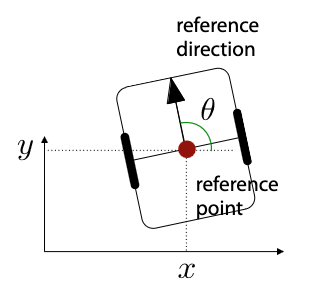
\includegraphics[width=.7\linewidth]{differential}
  %   \caption{$q=(x,y,\theta)$}\label{Fig:Data1}
  % \end{minipage}\hfill
  % \begin{minipage}{0.48\textwidth}
  %   \centering
  %   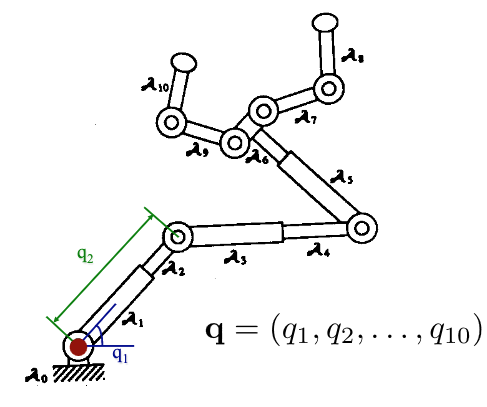
\includegraphics[width=.7\linewidth]{links}
  %   \caption{$q=(q{1},q_{2},...,q_{10})$}\label{Fig:Data2}
  % \end{minipage}
  %\end{figure}

\textbf{Espacio de configuraciones}: Es el espacio de todas las posibles configuraciones.\\

%\begin{figure}[!htb]
%   \begin{minipage}{0.48\textwidth}
%     \centering
%     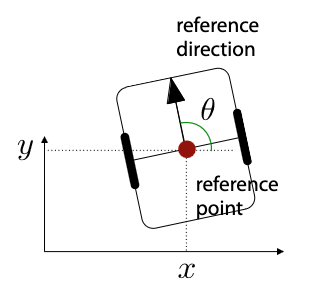
\includegraphics[width=.7\linewidth]{differential}
%     \caption{$q=(x,y,\theta)$}\label{Fig:Data3}
%   \end{minipage}\hfill
%   \begin{minipage}{0.48\textwidth}
%     \centering
%     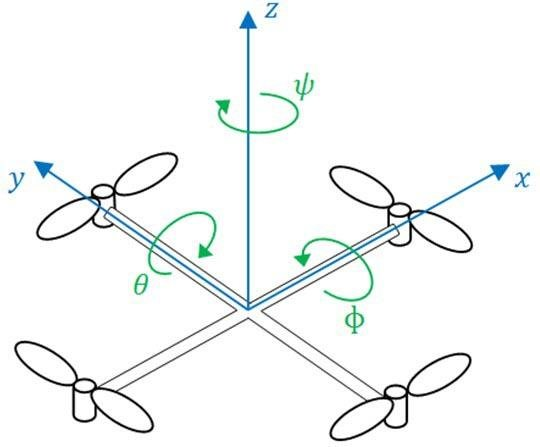
\includegraphics[width=.7\linewidth]{multirotor}
%     \caption{$q=(q{1},q_{2},...,q_{10})$}\label{Fig:Data4}
%   \end{minipage}
%\end{figure}

Es el espacio de configuraciones esta compuesto por los espacios libres ($C_{free}$) y espacios ocupado (con obstaculos) $C_{obs}$.\\

Sea $\mathcal{W} = \mathbb{R}^{m}$, $\mathcal{O} \in \mathcal{W}$ el conjunto de obstaculos, $\mathcal{A}(q)$ las configuraciones del robot $q \in \mathcal{C}$

\begin{itemize}
  \item $C_{free} = \{q \in \mathcal{C}|\mathcal{A}(q)\cap\mathcal{O} = \emptyset\}$
  \item $C_{obs} = C/C_{free}$
\end{itemize}

donde $\mathcal{W} = \mathbb{R}^{m}$ es el espacio de trabajo del robot, $\mathcal{O} \in \mathcal{W}$ es el conjunto de obstaculos, y $\mathcal{A}(q)$ son las configuraciones del robot $q \in \mathcal{C}$ .\\

Com\'{u}nmente se relaciona al problema de planificaci\'{o}n de rutas con el problema del mover un piano (\textbf{piano movement problem}). Es un problema dif\'{i}cil ya que el piano es un objeto en $\mathbb{R}^{3}$ que puede rotar y trasladarse. La \textbf{planificaci\'{o}n de rutas}, es similar. Ya que queremos mover al robot a un punto especifico.\\

En problemas cl\'{a}sicos de planificaci\'{o}n de rutas decimos que el camino \'{o}ptimo es el camino m\'{a}s corto, hay distintas formas cualitativas de poder ver un camino corto (Minimizando la energ\'{i}a en la trayectoria ..etc).\\

Nuestra soluci\'{o}n se centra en buscar la posible manera m\'{a}s r\'{a}pida de llegar de un punto al otro.\\

La planificaci\'{o}n de rutas presenta diversos retos:
\begin{itemize}
\item Restricciones fisicas del robot (su geometr\'{i}a o forma)
\item Din\'{a}mica del robot
\item Incertidumbres de lecturas de sensores (ruido)
\end{itemize}

Para crear rutas seguras, debemos respetar las restricciones para que el robot pueda ejecutar los movimientos en el mundo real.\\

Entonces, si le ordenamos al robot que ejecute una acci\'{o}n particular a trav\'{e}s de su interfaz de control, \textquestiondown qu\'{e} tan seguros estaremos de que el robot realmente lleg\'{o} a ese punto sin estar observandolo?\\

Los problemas que emergen de la planificaci\'{o}n de trayectorias es la \textbf{escalabilidad} y \textbf{eficiencia computacional}.\\

Considerando mover un VANT en 3D que puede trasladarse y rotar. El problema ser\'{a} en optimizar varios parametros por los 6 DoF (Grados de libertad) que cuenta y si queremos algoritmos que corran en tiempo real (que se ejecuten r\'{a}pido) dentro de dispositivos computacionales limitados.\\

Finalmente habr\'{a} obst\'{a}culos o otros robots en el ambiente que nuestra soluci\'{o}n de arquitectura deba considerar en su planificaci\'{o}n. El robot debe sensar los obst\'{a}culos y evitarlos.\\

\subsection*{Robots aereos}

UAVs are typically categorized as fixed-wing, rotary-wing, and hybrid-wing. Fixed-wing UAVs have rigid wings, like conventional human aircraft. They require relative velocity to generate aerodynamic forces and are thus more aero-dynamically efficient; however, fixed-wing UAVs require a runway for takeoff and landing. Vertical takeoff and landing are possible for rotary-wing UAVs because their revolving rotary blades generate adequate aerodynamic thrust. \cite{10120941}

Mostrar la figura 1 de \cite{10120941}, mostrar la figura 2 \cite{10120941}\\
Mostrar la tabla 5 \cite{10120941}

Claramente los problemas inherentes al control de vehiculos aereos son diferentes a los que pueda presentar un robot en tierra. Y su control recae en el ajuste de los angulos presentes en los tres ejes (roll, pitch, yaw).\\
  
  Millones de Veh\'{i}culos A\'{e}reos No Tripulados, o tambi\'{e}n conocidos como drones, han presentado una adopci\'{o}n masiva en diferentes aplicaciones, desde usos civiles (b\'{u}squeda y rescate, monitoreo industrial, vigilancia), hasta aplicaciones militares \cite{UAVCIVIL2019}. La popularidad de los VANT es atribuida a su movilidad.\\

La idea de utilizar m\'{u}ltiples robots a\'{e}reos en un sistema coordinado se basa en el comportamiento de los enjambres de animales, como las abejas o los p\'{a}jaros, que trabajan juntos de manera colaborativa para lograr objetivos comunes. Esta inspiraci\'{o}n biol\'{o}gica ha llevado al desarrollo de algoritmos y t\'{e}cnicas para coordinar y controlar m\'{u}ltiples VANT en diferentes aplicaciones.\\
  
  El inter\'{e}s en la investigaci\'{o}n e inovaci\'{o}n de soluciones con Veh\'{i}culos A\'{e}reos No Tripulados ha crecido exponencialmente en a\~{n}os recientes \citenum{Daponte2015,UAVPRACTICAL2023,GUPTA2016,VEGETACION2017,ROADS2017}.\\
  
  En recientes a\~{n}os, dotar a los VANT de inteligencia para explotar la informaci\'{o}n recolectada de sensores a bordo, ha sido y es un \'{a}rea estudiada en rob\'{o}tica m\'{o}vil \'{a}rea (construcci\'{o}n de mapas)\citenum{SHUKLA2016490}.\\

  Buscando probar diferentes teor\'{i}as de control, convirti\'{e}ndo los problemas t\'{i}picos de control 2D (p\'{e}ndulo inverso fijo) a un ambiente 3D, teniendo m\'{a}s variables a controlar para mantener el equilibrio del p\'{e}ndulo y al mismo tiempo lograr el movimiento y las maniobras deseadas del dron en el espacio tridimensional \citenum{PENDU2011}.\\
  
  El despliegue r\'{a}pido de robots en situaciones de riesgo, b\'{u}squeda y rescate ha sido un \'{a}rea ampliamente estudiada en la rob\'{o}tica m\'{o}vil. Donde existen concursos DARPA CHALLENGE donde todos los factores como exploraci\'{o}n, planeaci\'{o}n y coordinaci\'{o}n son clave para lograr los objetivos del Reto  \citenum{DARPA2022}. %se han aplicado teor\'{i}as de grafos para la obtenci\'{o}n de la mejor ruta. Los comportamientos reactivos son primordiales si pensamos en un agente aut\'{o}nomo.\\ %Esa percepci\'{o}n que podemos tener los seres humanos para reaccionar a ciertos retos. Buscar la manera de crear una arquitectura de software tolerante a fallas, capaz de coordinar m\'{u}ltiples v\'{e}hiculos a\'{e}reos no trupulados a medida que incrementa o disminuye la oferta de VANT(s) disponibles.\\

\subsection*{Panorama de m\'{e}todos de planificaci\'{o}n}

Un modelo del entorno nos ayudar\'{a} a conocer sus variables y reducir rutas inecesarias y asi el computo necesario. Metodos para modelar el ambiente se basan en aproximaciones de espacios, espacios libres, descomposicion por celdas, mapas topologicos y metodos probabilisticos como el PRM (probabilistic roadmap method).\\

Dentro del survey Path Planning for the Mobile Robot\citenum{sym10100450} muestran que el n\'{u}mero de publicaciones para planificadores de trayectoria, los algoritmos basados en Inteligencia Artificial han ganado terreno como soluciones para planificaci\'{o}n de rutas. Esto es en la b\'{u}squeda de la mejor en base a un mapa ya conocido.\\

Por otra parte el suvey de \cite{PathPlanning2020} se centra en los planificadores de rutas para VANT haciendo tres clasificaciones: T\'{e}cnicas por representacion, t\'{e}cnicas cooperativas y t\'{e}cnicas no cooperativas.\\

The path planning problem for UAVs is implemented as an optimization problem such that it gains an optimal solution among all the possible ones. There is no exact algorithm that defines an optimal path for the UAVs. The methods and algorithms for these path planning techniques are used to find the exact behavior of the UAVs for finding an optimal solution. \cite{PathPlanning2020}.

Los procesos m\'{a}s comunes para planificaci\'{o}n son:

\begin{itemize}
\item Representaci\'{o}n del VANT en un entorno 3D mostrando los obstaculos y el espacio libre.
\item Creaci\'{o}n del mapa o grafo que considere la configuraci\'{o}n y especificaciones del VANT en un entorno 3D.
\end{itemize}

\cite{XU2023110164} mencionan que la planificaci\'{o}n de trayectorias para multiples VANT es inherente a lo complejo del entorno y los trayectorias que pueda tomar el VANT. La minimizaci\'{o}n de la longitud de las rutas, configuraciones que pueda realizar el VANT y la seguridad del trayecto para todos los multi-VANT durante el vuelo son partes clave cuando se crea un planificador multi-VANT.\\

Apesar de las aproximaciones los planificadores globales se deben descomponer para poder considerar la existencia de obstaculos haciendo que la comunicaci\'{o}n entre ellos pueda ser afectada.\\

Tomando como ejemplo uno de sus deseables usos aut\'{o}nomos para b\'{u}squeda y rescate, supongamos que un VANT encuentra el objetivo, informa a los dem\'{a}s VANT para que vengan a ayudar lo m\'{a}s r\'{a}pido posible, la comunicaci\'{o}n entre ellos no debe perderse para lograr completar la tarea.\\
Es por ello que el conocimiento de algoritmos capaces de planear rutas cooperativas debe ser considerados.\\

En \'{u}ltimas decadas se han propuesto diversas tecnicas \textbf{metodos de programacion matematica (Mixed Integer Linear Programming (MILP), Nonlinear programming (NP) y Programaci\'{o}n din\'{a}mica (DP))} teniendo estos m\'{e}todos una fuerte base en teoria matematica. A pesar de ello estos metodos de programacion matem\'{a}tica su escala computacional crece exponencialmente conforme el espacio de b\'{u}squeda \cite{XU2023110164}.\\ 

Otros metodos que han sido ampliamente trabajados son los de Campo de Potencial Artificial ampliamente usado como planificador de trayectorias por sus ventajas en tiempo real. Desafortunadamente cuando existen dos campos de repulsion causados por obstaculos son iguales, este metodo cae en minimos locales llegando a fallar en encontrar una solucion.\\

Tambien se han propuesto los algoritmos basados en grafos para resolver el problema de planificaci\'{o}n de trayectorias.\\
Diagramas de Voronoi y el algoritmo A* siguen demostrando en encontrar efectivamente una ruta dependiendo de la division del espacio de busqueda. Estos metodos basados en grafos que funcionan muy bien en ambientes representados en 2D, pero al aplicarse a 3D toman mucho tiempo de ejecucion cuando el espacio de busqueda es complejo \citenum{DENG2023}.\\

Varios metodos de Inteligencia Computacional se han propuesto para el problema de planificaci\'{o}n de trayectorias (Algoritmos Geneticos GA, Ant Colony Optimization (ACO) \citenum{ZHAO2020}, Particle Swarm Optimization (PSO) y Evolucion Diferencial (DE). Estos algoritmos han demostrado crear rutas navegables para los VANT y son apliamente usados para problemas de planificacion de rutas complejos. Trabajos de \cite{DENG2023} han realizado adaptaciones al algoritmo PSO mostrado mejores resultados evitando caer en minimos locales con ayuda de Algoritmos Geneticos (GA) considerando parametros como inercia, funciones de activacion para la probabilidad de cruza y mutacion para los algoritmos geneticos han mostrado mejorar a rutas mas rapidas y estables.\\



%\begin{itemize}
%  \item Geom\'{e}tricos
%    \begin{itemize}
%    \item Grafos de visibilidad, descomposici\'{o}n en celdas, diagramas de voronoi, etc.
%    \end{itemize}
%  \item Campos de potencial
%    \begin{itemize}
%    \item Frentes de onta, funciones de navegaci\'{o}n, etc.
%    \end{itemize}
%  \item Basados en b\'{u}squeda
%    \begin{itemize}
%    \item Dijkstra, A*, D*, D* Lite, etc.
%    \end{itemize}
%  \item Basados en pruebas
%    \begin{itemize}
%    \item RRT, RRT*, PRM, etc.
%    \end{itemize}
%  \item Trayectorias
%    \begin{itemize}
%    \item M\'{i}nimo tiempo/energia, etc.
%    \end{itemize}
%  \item Bioinspirados
%    \begin{itemize}
%    \item Redes Neuronales, Algoritmos Geneticos, Ant Colony Optimisation, etc.
%    \end{itemize}
%\end{itemize}

La siguiente tabla muestra los m\'{e}todos de planificaci\'{o}n de trayectorias.\\

  \begin{tabular}{ |p{2cm}|p{1.5cm}|p{1.5cm}|p{1.4cm}|p{6cm}|  }
    \hline
    \tiny Metodo& \tiny Completez & \tiny \'{O}ptimo& \tiny Escalable& \tiny Notas \\
    \hline
    \rowcolor{black!5}
    \tiny Grafo de visibilidad   & \tiny Si    & \tiny Si&  \tiny No&
    \begin{itemize}[leftmargin=*, noitemsep, topsep=0pt]
    \tiny \item Mucho espacio libre
    \tiny \item Mala escalabilidad
    \tiny \item El robot pasa cerca de obstaculos
    \end{itemize}\\
    \hline
    \tiny Voronoi   & \tiny Si    & \tiny No& \tiny No&
    \begin{itemize}[leftmargin=*, noitemsep, topsep=0pt]
    \tiny \item Espacio libre m\'{a}ximo
    \tiny \item Rutas conservadoras
    \tiny \item Mala escalabilidad
    \end{itemize}\\
    \hline
    \rowcolor{black!5}
    \tiny Potential field   & \tiny Si    & \tiny No& \tiny Depende del ambiente&
    \begin{itemize}[leftmargin=*, noitemsep, topsep=0pt]
    \tiny \item Depende del ambiente
    \tiny \item F\'{a}cil de implementar
    \tiny \item Suceptible a m\'{i}nimos locales
    \end{itemize}\\
    \hline
    \tiny Dijkstra/A*   & \tiny Si    & \tiny Grid& \tiny No&
    \begin{itemize}[leftmargin=*, noitemsep, topsep=0pt]
    \tiny \item M\'{a}s r\'{a}pido que la b\'{u}squeda desinformada
    \tiny \item A* usa una funci\'{o}n heur\'{i}stica para impulsar la b\'{u}squeda de manera eficiente
    \tiny \item Mala escalabilidad
    \end{itemize}\\
    \hline
    \rowcolor{black!5}
    \tiny PRM   & \tiny Si    & \tiny Grafo& \tiny Si&
    \begin{itemize}[leftmargin=*, noitemsep, topsep=0pt]
    \tiny \item Eficiente para problemas con consultas múltiples
    \tiny \item Completez probabil\'{i}stica\
    \tiny \item Camino irregular
    \end{itemize}\\
    \hline
    \tiny RRT   & \tiny Si    & \tiny No & \tiny Si&
    \begin{itemize}[leftmargin=*, noitemsep, topsep=0pt]
    \tiny \item Eficiente para problemas de consulta \'{u}nica
    \tiny \item Completez probabil\'{i}stica
    \tiny \item Camino irregular
    \end{itemize}\\
    \hline
  \end{tabular}


%%%%%%%%%%%%%%%%%%%%%%%%%%%
% IMAGEN Sistema autonomo
%%%%%%%%%%%%%%%%%%%%%%%%%%%

%\begin{itemize}
%\item Hablar de la robotica de servicios
%\item robotica movil
%\item clasificar los diversos robots moviles aereos
%\item los problemas en la robotica movil
%\item slam
%\item robots coolaborativos
%\end{itemize}

%%%%%%%%%%%%%%%%%%%%%%%%%%%

%%%%%%%%%%%%%%%%%%%%%%%%%%%

%\noindent\makebox[\linewidth]{\rule{\paperwidth}{0.4pt}}

%\begin{center}
%\fbox{\parbox[t]{14em}{
%    \begin{itemize}
%      \tiny \item Caracteristicas Robot
%      \begin{itemize}
%        \tiny \item Grados de libertad
%        \tiny \item Fisica del robot
%        \tiny \item limitaciones en Mobilidad
%        \tiny \item limitaciones en Dinamica
%      \end{itemize}
%    \end{itemize}
%  }
%}%
%\raisebox{-10ex}{\Huge$\to$}%
%\fbox{\parbox[t]{14em}{
%    \begin{itemize}
%      \tiny \item Propiedades del algortimo
%      \begin{itemize}
%        \tiny \item Optimalidad
%        \tiny \item Costo Computacional
%        \tiny \item Costo en memoria
%        \tiny \item Completez
%        \tiny \item Online vs. Offline
%        \tiny \item Anytime
%        \tiny \item Caminos vs. trayectorias
%        \tiny \item Exactos vs. aproximados
        
%      \end{itemize}
%    \end{itemize}
%  }
%}
%\end{center}

\newpage
\section*{Planteamiento del problema}

%The problem addressed can be summarized as follows: Given a bounded 3D-volume V that an agent e.g. a drone wishes to explore, which actions should the agent perform to explore V completely and as fast as possible? Each point in this volume, $x∈V⊂R3$, can take the two values: free or occupied, i.e. V(x)=(free|occupied).\\

%Complete exploration means that the agent has created a map M covering the volume V and every point x in the map, that can be observed by any of the agent's sensors, has been observed as free or occupied, i.e. M(xreachable)=(free|occupied). Points that are non-observable, e.g. hollow spaces without openings, the inside of thick walls or space out of range, will still be unmapped even after the exploration has been completed. If no prior information is given, every x in the map is initially unmapped. Due to the active nature of the problem, it has to be solved online.\\

La coordinaci\'{o}n de m\'{u}ltiples-VANT (Veh\'{i}culos A\'{e}reos No Tripulados) es un desaf\'{i}o complejo en el campo de la rob\'{o}tica y la exploraci\'{o}n de \'{a}reas desconocidas. A medida que la tecnolog\'{i}a de los Veh\'{i}culos A\'{e}reos No Tripulados contin\'{u}a avanzando y se vuelven m\'{a}s accesibles, se presenta la oportunidad de utilizar equipos de m\'{u}ltiples VANT para realizar tareas de manera colaborativa y eficiente. Sin embargo, esta coordinaci\'{o}n planea diversas problem\'{a}ticas que deben abordarse.\\

La coordinaci\'{o}n de m\'{u}ltiples VANT implica la necesidad de establecer una comunicaci\'{o}n efectiva entre ellos. Los VANT deben intercambiar informaci\'{o}n relevante sobre su posici\'{o}n, estado, objetivos y otros datos importantes. La comunicaci\'{o}n debe ser confiable, de baja latencia y capaz de manejar m\'{u}ltiples enlaces de manera simult\'{a}nea. Adem\'{a}s, los protocolos de comunicaci\'{o}n deben ser seguros para proteger la integridad y confidencialidad de los datos transmitidos.\\

Otro desaf\'{i}o es la planificaci\'{o}n de rutas y la toma de decisiones distribuida. Los VANT deben coordinar sus movimientos para evitar colisiones y lograr una cobertura eficiente del \'{a}rea objetivo. Esto implica la necesidad de desarrollar algoritmos y estrategias que permitan la planificaci\'{o}n de rutas din\'{a}micas, considerando los obst\'{a}culos y las restricciones del entorno. Adem\'{a}s, los VANT deben tomar decisiones colaborativas para adaptarse a situaciones imprevistas o cambios en el entorno.\\

La asignaci\'{o}n de tareas tambi\'{e}n es un aspecto cr\'{i}tico en la coordinaci\'{o}n de m\'{u}ltiples VANT. Cada VANT puede tener diferentes capacidades y sensores especializados, por lo que es importante asignar tareas de acuerdo con las fortalezas individuales de cada robot. Adem\'{a}s, los VANT deben colaborar en la recolecci\'{o}n y procesamiento de datos, evitanto la duplicaci\'{o}n de esfuerzos optimizando el uso de los recursos disponibles.\\

Dada un \'{a}rea de inter\'{e}s $A$ desconocida que se desea explorar,

\begin{itemize}
\item Un conjunto de Veh\'{i}culos A\'{e}reos No Tripulados (VANT) denotados como $V = V_{1},V_{2},V_{3},...,V_{n}$, donde $n$ es el n\'{u}mero total de VANT's disponibles
\item Un conjunto de tareas de exploraci\'{o}n denotados como $T = T_{1}, T_{2}, T_{3}, T_{m}$, donde $m$ es el n\'{u}mero total de tareas a realizar.
\end{itemize}

restricciones y requisitos espec\'{i}ficos del problema, como l\'{i}mites de tiempo, obst\'{a}culos a evitar. Para cada tarea de exploraci\'{o}n $T_{m}$, se definen las siguientes variables:

\begin{itemize}
\item Posici\'{o}n inicial: $p_{i}(x,y,z)$, representa la posici\'{o}n inicial del VANT o los m\'{u}ltiples-VANTs asignados a la tarea $T_{m}$
\item Trayectoria: $\alpha_{i}$, describe la trayectoria seguida por el/los VANT asignado(s) a la tarea $T_{m}$ en funci\'{o}n del tiempo $t$
\item Informaci\'{o}n recolectada: $C_{i}$, representa la informaci\'{o}n recolectada por el/los VANT asignado(s) durante la exploraci\'{o}n
\end{itemize}

La funci\'{o}n objetivo variar\'{a} seg\'{u}n los objetivos espec\'{i}ficos del problema.
\begin{itemize}
\item Maximizar la cobertura del \'{a}rea de inter\'{e}s $A$
\item Minimizar el tiempo total requerido para cubrir el \'{a}rea de inter\'{e}s $A$
\item Maximizar la cantidad de informaci\'{o}n recolectada
\end{itemize}

Con base en lo anterior, surgen las siguientes preguntas de investigaci\'{o}n:

\begin{itemize}
\item \textquestiondown Cual\'{e}s son los mejores algoritmos conocidos adecuados para correr en una tarjeta electr\'{o}nica con recursos limitados?
\item \textquestiondown Es posible crear una arquitectura de software capaz de coordinar m\'{u}ltiples-VANTS para tareas en exploraci\'{o}n de manera eficiente?
\end{itemize}

\subsection*{Hip\'{o}tesis}

Es posible crear una arquitectura de software para coordinar multiples-VANTS en exploracion que sea de orden lineal capaz de contar con una representacion del ambiente en voxels.

\section*{Objetivos generales y espec\'{\i}ficos del proyecto}

\textbf{General} \\

Dise\~{n}ar una arquitectura de software descentralizada capaz de resolver los problemas de localizaci\'{o}n, mapeo, navegaci\'{o}n y coordinaci\'{o}n multi-VANT en ambientes desconocidos y din\'{a}micos para tareas de exploraci\'{o}n en interiores.

%Desarrollo e implementaci\'{o}n de una arquitectura de software tolerante a fallas para la coordinaci\'{o}n de m\'{u}ltiples VANT(s) aplicados a una simulaci\'{o}n de b\'{u}squeda y rescate.

%El objetivo general de la tesis es desarrollar estrategias efectivas para la coordinación de m\'{u}ltiples Veh\'{i}culos A\'{e}reos no Tripulados, con el fin de mejorar la eficiencia y el rendimiento en aplicaciones en exploraciones aéreas.

\bigskip
\noindent
%\textbf{Particulares} \\
De manera m\'{a}s espec\'{i}fica, se listan los siguientes objetivos: %espec\'{i}ficos:

\begin{enumerate}

\item \textbf{Construcci\'{o}n propuesta} Evaluar las soluciones en la literatura asociados con la coordinaci\'{o}n multi-VANT. Enfoc\'{a}ndose en aspectos como la comunicaci\'{o}n, evasi\'{o}n de obst\'{a}culos, asignaci\'{o}n de tareas y sincronizaci\'{o}n de informaci\'{o}n. En base a esta valoraci\'{o}n, construir una arquitectura de software para la coordinaci\'{o}n multi-VANT.

\item \textbf{Valoraci\'{o}n (prueba) propuesta} Emplear una herramienta de simulaci\'{o}n de libre uso para rob\'{o}tica, para el desarrollo y puesta en marcha de una propuesta de arquitectura de software capaz de realizar el control multi-VANT y evaluar el desemple\~{n}o de dicha arquitectura.
  
\item \textbf{Comparaci\'{o}n y an\'{a}lisis} Comparar y analizar los resultados obtenidos con enfoques existentes en la coordinaci\'{o}n multi-VANT, mostrando las ventajas y desventajas de la estrategia propuesta. Con base a estos an\'{a}lisis proponer recomendaciones y pautas pr\'{a}cticas para la implementaci\'{o}n y aplicaci\'{o}n de la estrategias de coordinaci\'{o}n multi-VANT en escenarios reales, considerando factores como la escalabilidad, la robustez y los recursos computacionales requeridos.

\end{enumerate}

\newpage
\section*{Metodolog\'{\i}a}

La metodolog\'{i}a propuesta se divide en tres etapas, iniciando en septiembre del 2023. A continuaci\'{o}n se detallan cada una de las actividades que se plantean realizar en cada una.

\subsection*{Etapa 1. An\'{a}lisis y dise\~{n}o de la soluci\'{o}n propuesta}

En esta etapa se comprende en la revisi\'{o}n de la literatura de manera m\'{a}s completa, que permita contar con la informaci\'{o}n necesaria para la elecci\'{o}n de los mejores algoritmos para abordar cada una de las problem\'{a}ticas asociadas con la coordinaci\'{o}n de trayectorias. Una vez realizada la elecci\'{o}n de los algoritmos que se usar\'{a}n para la propuesta de arquitectura de software, se proceder\'{a} a revisar y estudiar las arquitecturas para los robots colaborativos. Finalmente, se realizar\'{a} el dise\~{n}o de la arquitectura.\\

Las actividades espec\'{i}ficas a realizarse en la etapa 1, son:
  
  \begin{enumerate}
  \item[] \textbf{E1.A1.} \textbf{Revisi\'{o}n estado del arte} Ampliar la revisi\'{o}n de la literatura sobre coordinaci\'{o}n y exploraci\'{o}n multi-VANT.
  \item[] \textbf{E1.A2.} \textbf{Evaluaci\'{o}n de aptitudes} Revisar y documentar los aspectos relevantes (asi como sus limitantes) que permiten la colaboraci\'{o}n, coordinaci\'{o}n y balanceo de la carga de trabajo multi-VANT.
  %\item \textbf{E1.A3.} \textbf{Selecci\'{o}n de algoritmos} Estudiar las limitantes de las soluciones relevantes en la literatura en base a autonomia e inteligencia computacional.
  \item[] \textbf{E1.A3.} \textbf{Selecci\'{o}n de algoritmos} Seleccionar los algoritmos para planificaci\'{o}n de trayectorias y exploraci\'{o}n en ambientes desconocidos representativos para un entorno de computaci\'{o}n restringida.
  \item[] \textbf{E1.A4.} \textbf{Elaboraci\'{o}n de soluci\'{o}n} Definir la arquitectura de software para escenarios en aplicaciones multi-VANT apegadas a las especificaciones de computadora de placa reducida (Raspberry Pi, Esp32 ... etc.).
  \item[] \textbf{E1.A5.} \textbf{Documentaci\'{o}n Etapa 1} Elaborar la documentaci\'{o}n de la revisi\'{o}n del estado del arte y del trabajo realizado que formar\'{a} parte de la tesis.
  \item[] \textbf{E1.A6.} \textbf{Revisi\'{o}n de tesis} Revisi\'{o}n y correcci\'{o}n de avances con los asesores.
  \end{enumerate}
  
  \subsection*{Etapa 2. Implementaci\'{o}n y validaci\'{o}n}
  
  Esta etapa se centra en el desarrollo e implementaci\'{o}n del dise\~{n}o de la arquitectura de software para la coordinaci\'{o}n multi-VANT.\\
  
  Las actividades espec\'{i}ficas a realizarse en la etapa 2, son:

  \begin{enumerate}
  \item[] \textbf{E2.A1.} \textbf{Selecci\'{o}n Simulador} Al tener definida la arquitectura de software y conocer las estructuras de datos que se utilizaran, evaluar los diversos simuladores para rob\'{o}tica de libre uso. (Revisar temas de modelos 3D, din\'{a}mica del robot, representaci\'{o}n del ambiente 3D, simulaci\'{o}n de sensores). 
  \item[] \textbf{E2.A2.} \textbf{Creaci\'{o}n modelo 3D} Crear un modelo 3D en base al simulador seleccionado apegandose a las dimensiones de un VANT que se pueda replicar.
  \item[] \textbf{E2.A3.} \textbf{Control de desplazamientos} Crear movimientos y control de un VANT y m\'{u}ltiples VANT, algoritmos que forman parte de la capa reactiva del VANT.
  \item[] \textbf{E2.A4.} \textbf{Desarrollo de visualizaci\'{o}n de datos} A partir de la selecci\'{o}n del sensor, se desarrollar\'{a} la forma de representar el entorno 3D dentro del simulador elegido.
  \item[] \textbf{E2.A5.} \textbf{Desarrollo de algoritmos de exploraci\'{o}n} En base a la revisi\'{o}n del estado del arte se implementar\'{a} el algoritmo propuesto para la exploraci\'{o}n con un VANT
  \item[] \textbf{E2.A6.} \textbf{Implementaci\'{o}n un solo VANT} Realizar pruebas y corregir errores en base a los desarrollos realizados.
  \item[] \textbf{E2.A7.} \textbf{Simulaci\'{o}n un solo VANT} Realizar pruebas de simulaci\'{o}n con un solo VANT de la soluci\'{o}n propuesta.
  \item[] \textbf{E2.A8.} \textbf{Desarrollo de coordinaci\'{o}n} Al contar con la exploraci\'{o}n y navegaci\'{o}n exitosa de un solo VANT, se procede al desarrollo de coordinaci\'{o}n multi-VANT.
  \item[] \textbf{E2.A9.} \textbf{Implementaci\'{o}n multi-VANT} Realizar pruebas y corregir errores en base a los desarrollos realizados para la coordinaci\'{o}n multi-VANT.
  \item[] \textbf{E2.A10.} \textbf{Simulaci\'{o}n multi-VANT} Realizar pruebas de simulaci\'{o}n multi-VANT de la soluci\'{o}n propuesta.
  \item[] \textbf{E2.A11.} \textbf{Documentaci\'{o}n Etapa 2} Elaborar la documentaci\'{o}n del desarrollo e implementaci\'{o}n de la propuesta de arquitectura de software para la coordinaci\'{o}n multi-VANT que formar\'{a} parte de la tesis.
  \item[] \textbf{E2.A12.} \textbf{Revisi\'{o}n de tesis} Revisi\'{o}n y correcci\'{o}n de cap\'{i}tulos con los asesores.
  \end{enumerate}
  

  \subsection*{Etapa 3. Evaluaci\'{o}n experimental, resultados y conclusiones}
  
  Partiendo del prototipo y las simulaciones desarrolladas en la etapa anterior, en esta etapa se realizan todas las actividades relacionadas con la evaluacion, recabacion de resultados y la escritura de los capitulos restantes de la tesis. Ademas se realizara el proceso de graduacion y actividades relacionadas.\\

  Las actividades espec\'{i}ficas a realizarse en la etapa 3, son:
  
  \begin{enumerate}
  \item[] \textbf{E3.A1.} \textbf{Experimentaci\'{o}n de soluci\'{o}n} Experimentos para evaluar el desempe\~{n}o de la solucion propuesta creada en la etapa anterior.  
  \item[] \textbf{E3.A2.} \textbf{Recopilaci\'{o}n de resultados} Recabar la informacion de los resultados, realizar su analisis y generar la documentacion correspondiente.
  \item[] \textbf{E3.A3.} \textbf{Documentaci\'{o}n Etapa 3} Elaborar la documentaci\'{o}n de los resultados obtenidos y conclusiones que formar\'{a} parte de la tesis.
  \item[] \textbf{E3.A4.} \textbf{Revisi\'{o}n de tesis} Revisi\'{o}n y correcci\'{o}n de tesis con los asesores.
  \item[] \textbf{E3.A5.} \textbf{Divulgaci\'{o}n} Escribir un art\'{i}culo cient\'{i}fico, con los hallazgos de esta tesis y participar en actividades de difusi\'{o}n.
  \item[] \textbf{E3.A6.} \textbf{Proceso de titulaci\'{o}n} Comenzar el proceso de titulaci\'{o}n
  \end{enumerate}
  
\section*{Cronograma de actividades (plan de trabajo)}

\begin{minipage}{11cm}
\noindent\begin{tabular}{|p{0.6\textwidth}*{12}{|p{0.040\textwidth}}|}
% The top line
%\diagbox[width=12.5em]{Actividades}{Cuatrimestres}
\hline

& \multicolumn{4}{c|}{\textbf{Cuatrimestre 1}} 
& \multicolumn{4}{c|}{\textbf{Cuatrimestre 2}}  
& \multicolumn{4}{c|}{\textbf{Cuatrimestre 3}}\\
\hline
% The second line, with its five years of four quarters
%\textcolor{black}{\textbf{Etapas}}
\rpt[3]{& 1 & 2 & 3 & 4} \\
\hline
\rowcolor{black!5}{\textbf{Etapa 1}}\\
% using the on macro to fill in twenty cells as `on'
%\specialcell{Actividad 1\\espacio}        \on[0] \off[12] \\
%Actividad 1    \on[0] \off[12]\\
\hline
\textbf{E1.A1.} Revisi\'{o}n estado del arte    \on[1] \off[11] \\
\hline
\textbf{E1.A2.} Evaluaci\'{o}n de aptitudes    \on[1]  \off[11] \\
\hline
\textbf{E1.A3.} Selecci\'{o}n de algoritmos    \on[2]  \off[10] \\
\hline
\textbf{E1.A4.} Elaboraci\'{o}n de soluci\'{o}n    \on[3]  \off[9] \\
\hline
\textbf{E1.A5.} Documentaci\'{o}n Etapa 1    \off[2] \on[1]  \off[9] \\
\hline
\textbf{E1.A6.} Revisi\'{o}n de tesis Etapa 1    \off[2] \on[1]  \off[9] \\
\hline
% using the on macro followed by the off macro
\rowcolor{black!5}{\textbf{Etapa 2}}\\
\hline
\textbf{E2.A1.} Selecci\'{o}n Simulador    \off[3] \on[1]  \off[8] \\
\hline
\textbf{E2.A2.} Creaci\'{o}n modelo 3D   \off[3] \on[1]  \off[8] \\
\hline
\textbf{E2.A3.} Control de desplazamientos  \off[3] \on[2]  \off[7] \\
\hline
\textbf{E2.A4.} Desarrollo de visualizaci\'{o}n de datos   \off[3] \on[2]  \off[7] \\
\hline
\textbf{E2.A5.} Desarrollo de algoritmos de exploraci\'{o}n  \off[3] \on[2]  \off[7] \\
\hline
\textbf{E2.A6.} Implementaci\'{o}n un solo VANT   \off[4] \on[1]  \off[7] \\
\hline
\textbf{E2.A7.} Simulaci\'{o}n un solo VANT  \off[4] \on[2]  \off[6] \\
\hline
\textbf{E2.A8.} Desarrollo de coordinaci\'{o}n  \off[5] \on[2]  \off[5] \\
\hline
\textbf{E2.A9.} Implementaci\'{o}n multi-VANT  \off[6] \on[1]  \off[5] \\
\hline
\textbf{E2.A10.} Simulaci\'{o}n multi-VANT \off[7] \on[1]  \off[4] \\
\hline
\textbf{E2.A11.} Documentaci\'{o}n Etapa 2  \off[7] \on[1]  \off[4] \\
\hline
\textbf{E2.A12.} Revisi\'{o}n de tesis  \off[7] \on[1]  \off[4] \\
\hline
\rowcolor{black!5}{\textbf{Etapa 3}}\\
\hline
\textbf{E3.A1.} Experimentaci\'{o}n de soluci\'{o}n   \off[8] \on[2]  \off[2] \\
\hline
\textbf{E3.A2.} Recopilaci\'{o}n resultados   \off[9] \on[1]  \off[2] \\
\hline
\textbf{E3.A3.} Documentaci\'{o}n Etapa 3  \off[10] \on[1]  \off[1] \\
\hline
\textbf{E3.A4.} Revisi\'{o}n de tesis \off[10] \on[2] \\
\hline
\textbf{E3.A5.} Divulgaci\'{o}n \off[6] \on[6] \\
\hline
\textbf{E3.A6.} Proceso de titulaci\'{o}n  \off[11] \on\\
\hline
\end{tabular}
\end{minipage}

\iffalse
\begin{ganttchart}[vgrid={draw=none, dotted}]{1}{12}
\gantttitlelist{1,...,12}{1} \\
\ganttbar{}{1}{4} \\
\ganttbar{}{5}{11}
\end{ganttchart}


\definecolor{barblue}{RGB}{153,204,254}
\definecolor{groupblue}{RGB}{51,102,254}
\definecolor{linkred}{RGB}{165,0,33}
\renewcommand\sfdefault{phv}
\renewcommand\mddefault{mc}
\renewcommand\bfdefault{bc}

\setganttlinklabel{s-s}{START-TO-START}
\setganttlinklabel{f-s}{FINISH-TO-START}
\setganttlinklabel{f-f}{FINISH-TO-FINISH}
\sffamily
\begin{ganttchart}[
    canvas/.append style={fill=none, draw=black!5, line width=.75pt},
    hgrid style/.style={draw=black!5, line width=.75pt},
    vgrid={*1{draw=black!5, line width=.75pt}},
    today=7,
    today rule/.style={
      draw=black!64,
      dash pattern=on 3.5pt off 4.5pt,
      line width=1.5pt
    },
    today label font=\small\bfseries,
    title/.style={draw=none, fill=none},
    title label font=\bfseries\footnotesize,
    title label node/.append style={below=7pt},
    include title in canvas=false,
    bar label font=\mdseries\small\color{black!70},
    bar label node/.append style={left=2cm},
    bar/.append style={draw=none, fill=black!63},
    bar incomplete/.append style={fill=barblue},
    bar progress label font=\mdseries\footnotesize\color{black!70},
    group incomplete/.append style={fill=groupblue},
    group left shift=0,
    group right shift=0,
    group height=.5,
    group peaks tip position=0,
    group label node/.append style={left=.6cm},
    group progress label font=\bfseries\small,
    link/.style={-latex, line width=1.5pt, linkred},
    link label font=\scriptsize\bfseries,
    link label node/.append style={below left=-2pt and 0pt}
  ]{1}{13}
  \gantttitle[
    title label node/.append style={below left=7pt and -3pt}
  ]{CUATRIMESTRE:\quad1}{1}
  \gantttitlelist{2,...,13}{1} \\
  \ganttgroup[progress=57]{WBS 1 Summary Element 1}{1}{10} \\
  \ganttbar[
    progress=75,
    name=WBS1A
  ]{\textbf{WBS 1.1} Activity A}{1}{8} \\
  \ganttbar[
    progress=67,
    name=WBS1B
  ]{\textbf{WBS 1.2} Activity B}{1}{3} \\
  \ganttbar[
    progress=50,
    name=WBS1C
  ]{\textbf{WBS 1.3} Activity C}{4}{10} \\
  \ganttbar[
    progress=0,
    name=WBS1D
  ]{\textbf{WBS 1.4} Activity D}{4}{10} \\[grid]
  \ganttgroup[progress=0]{WBS 2 Summary Element 2}{4}{10} \\
  \ganttbar[progress=0]{\textbf{WBS 2.1} Activity E}{4}{5} \\
  \ganttbar[progress=0]{\textbf{WBS 2.2} Activity F}{6}{8} \\
  \ganttbar[progress=0]{\textbf{WBS 2.3} Activity G}{9}{10}
  \ganttlink[link type=s-s]{WBS1A}{WBS1B}
  \ganttlink[link type=f-s]{WBS1B}{WBS1C}
  \ganttlink[
    link type=f-f,
    link label node/.append style=left
  ]{WBS1C}{WBS1D}
  \end{ganttchart}
\fi

\section*{Infraestructura}

Para el desarrollo de este proyecto de investigaci\'{o}n, se har\'{a} uso de un equipo de c\'{o}mputo con las siguientes caracter\'{i}sticas:

\begin{itemize}
\item iMac (21.5-inch, Late 2015)
\item Procesador 2.8 GHz Quad-Core Intel Core i5
\item Memoria Ram 8 GB 1867 MHz DDR3
\item Graphics Intel Iris Pro Graphics 6200 1536 MB
\item Almacenamiento 1 TB
\end{itemize}

\newpage
\section*{Estado del arte}

%\begin{vtimeline}[description={text width=7cm}, 
% row sep=4ex, 
% use timeline header,
% timeline title={The title}]
%1947 & AT and T Bell Labs develop the idea of cellular phones\endlr
%1968 & Xerox Palo Alto Research Centre envisage the `Dynabook'\endlr
%1971 & Busicom 'Handy-LE' Calculator\endlr
%1973 & First mobile handset invented by Martin Cooper\endlr
%1978 & Parker Bros. Merlin Computer Toy\endlr
%1981 & Osborne 1 Portable Computer\endlr
%1982 & Grid Compass 1100 Clamshell Laptop\endlr
%1983 & TRS-80 Model 100 Portable PC\endlr
%1984 & Psion Organiser Handheld Computer\endlr
%1991 & Psion Series 3 Minicomputer\endlr
%\end{vtimeline}

%\begin{vtimeline}[timeline color=cyan!80!blue, add bottom line, line offset=2pt]
%1947 & AT and T Bell Labs develop the idea of cellular phones\endlr
%1968 & Xerox Palo Alto Research Centre envisage the `Dynabook'\endlr
%1971 & Busicom 'Handy-LE' Calculator\endlr
%1973 & First mobile handset invented by Martin Cooper\endlr
%1978 & Parker Bros. Merlin Computer Toy\endlr
%1981 & Osborne 1 Portable Computer\endlr
%1982 & Grid Compass 1100 Clamshell Laptop\endlr
%1983 & TRS-80 Model 100 Portable PC\endlr
%1984 & Psion Organiser Handheld Computer\endlr
%1991 & Psion Series 3 Minicomputer\endlr
%\end{vtimeline}

En el Centro de Investigaci\'{o}n y Estudios Avanzados del Institudo Polit\'{e}cnico Nacional Unidad Tamaulipas se han realizado investigaciones en el \`{a}rea de exploraci\'{o}n multi-robot y dise\~{n}o de prototipos de VANTS, lo cual sirve como antecedente para este trabajo.\\

Entre los trabajos m\'{a}s relevantes se encuentra la tesis doctoral de \cite{CINVESTAM2013} que tiene como objetivo general el dise\~{n}o e implementaci\'{o}n de la coordinaci\'{o}n de multi-robot con un enfoque de auto-ofertas\\

Por otra parte trabajos de tesis de maestria de \cite{CINVES2013} que tiene como objetivo general la Generaci\'{o}n de mapas utilizando veh\'{i}culos a\'{e}reos no tripulados de baja altitud.\\

Este trabajo desarrolla usando una combinacion entre la tecnica y tecnica de ... en especial el algoritmo de ... Los resultados de este trabajo muestran un buen desempe\~{n}o del sistema de control....
La robustez se alcanza para las perturbaciones.\\

Otra investigacion relevante se encuentra en la tesis de doctorado del CINVESTAV Unidad Guadalajara \cite{CINVES2021, CINVES2015}.
El objetivo principal de este trabajo es el de realizar seguimiento ..\\

%sacar notas para clase de http://srl.informatik.uni-freiburg.de/teachingdir/ws13/slides/12-RobotMotionPlanning.pdf
%https://msl.cs.uiuc.edu/planning/node158.html

Recopilacion de algoritmos Sampling-based algorithms for optimal motion planning \cite{Karaman2011}\\

Exploration pioneering research points to seminal work done by [10] introducing a frontier-based approach. A frontier distinguishes the boundary line between explored and unexplored regions on the map. During robot navigation the environment information gathered increases constantly, thus pushing the frontier boundary further until no frontiers are left. Such strategies have been widely tested on Unmanned Ground Vehicles (UGV) [11][13] in simple environments having 3 - Degrees-of-Freedom (DoF) i.e., (x, y, $\theta$) whereas a UAV can maneuver in more complex 3D environments with a pose of 6 - DoF, i.e., transitional and rotational positions to control the UAV. \cite{9836079}\\

Multi-Vehicle Motion Planning for Search and Tracking \cite{8397034}\\
Multiobjective UAV Path Planning for Emergency Information Collection and Transmission \cite{9031752}\\
Research on Dynamic Obstacle Avoidance Path Planning Strategy of UAV \cite{9986687}\\
Integrating Local Motion Planning and Robust Decentralized Fault-Tolerant Tracking Control for Search and Rescue Task of Hybrid UAVs and Biped Robots Team System \cite{10120943}\\
An End-to-End Deep Reinforcement Learning Method for UAV Autonomous Motion Planning \cite{10056204}\\
Self-organized search-attack mission planning for UAV swarm based on wolf pack hunting behavior \cite{9679714}\\
Short and Full Horizon Motion Planning for Persistent multi-UAV Surveillance with Energy and Communication Constraints \cite{9679714}\\
A Study on UAV Formation Collision Avoidance \cite{8028745}\\
Application of Motion Planning in UAVs: A Review \cite{10055974}\\
A 3D path planning approach for quadrotor UAV navigation \cite{7279703}\\
Coverage Path Planning Optimization of Heterogeneous UAVs Group for Precision Agriculture \cite{10011226}\\
Unmanned aerial vehicle navigation in underground structure inspection: A review \cite{Zhang2023}\\
Transmission Line Inspection Using Unmanned Aerial Vehicle \cite{Subahani2020}\\
Decentralized Spatial-Temporal Trajectory Planning for Multicopter Swarms \cite{zhou2021decentralized}\\
A Survey on multi-robot systems \cite{6320878}\\
Sacar mas paha de aca? \cite{DENG2023}\\
talves de aca mas paha \cite{UAVPRACTICAL2023}\\
hojeada de aca \cite{XU2023110164}
%https://docs.ufpr.br/~danielsantos/ProbabilisticRobotics.pdf

revisar: \cite{drones7060337}\\
sacar mas data de aqui \cite{PathPlanning2020} y de aca \cite{10120941} y de aca \cite{UAVPRACTICAL2023} o de aca \cite{ZOUGANELI2022}, revisar \cite{math11102356}\\
Dar revisada a \cite{CHEN2014}\\


Las aplicaciones de la rob\'{o}tica se han centrado en realizar tareas simples y repetitivas. La necesidad de robots con capacidad de identificar cambios en su entorno y reaccionar sin la intervenci\'{o}n humana, da origen a los robots inteligentes. Aunado a ello si deseamos que el robot se mueva libremente, los cambios en su entorno pueden aumentar r\'{a}pidamente y complicar el problema de un comportamiento inteligente. Dentro de la rob\'{o}tica m\'{o}vil inteligente se han propuesto estrategias de comportamiento reactivas, algoritmos que imitan el comportamiento de insectos y el c\'{o}mo se desplanzan en un entorno.\\
El objetivo principal de los algoritmos de navegaci\'{o}n es el de guiar al robot desde el punto de inicio al punto destino. Los trabajos por V. Lumelsky y A. Stephanov, et al. [11], dieron respuesta a problematicas de navegaci\'{o}n eficiente y de poca memoria (Algoritmos tipo bug).\\
Se considera a P. Hart, N. Nilsson et al. como los creadores del algoritmo A* en 1968 [12], al mejorar el algoritmo de Dijkstra para el robot Shakey, que deb\'{i}a navegar en una habitaci\'{o}n que conten\'{i}a obst\'{a}culos fijos. El objetivo principal del algoritmo A* es la eficiencia en la planificaci\'{o}n de rutas.\\
Otros algoritmos propuestos por A. Stentzz[13] han demostrado operar de manera eficiente ante obst\'{a}culos din\'{a}micos, a comparaci\'{o}n del algoritmo A* que vuelve a ejecutarse al encontrarse con un obst\'{a}culo, el algoritmo D* usa la informaci\'{o}n previa para buscar una ruta hacia el objetivo.\\

%La planificación de trayectorias también ha abordado la problemática de la planificación de múltiples robots. Se han desarrollado algoritmos que permiten a los robots colaborar y coordinarse para evitar colisiones y mejorar la eficiencia en sus tareas. Estos enfoques utilizan técnicas de planificación centralizada o descentralizada, y pueden basarse en métodos de búsqueda o algoritmos de optimización multiobjetivo.\\

La colaboraci\'{o}n de m\'{u}ltiples VANTs (veh\'{i}culos a\'{e}reos no tripulados), tambi\'{e}n conocidos como VANTs, ha surgido como una \'{a}rea de investigaci\'{o}n prometedora en los \'{u}ltimos a\~{n}os [1,2,3,5]. La capacidad de coordinar y colaborar entre s\'{i} permite a los VANTs realizar tareas complejas de manera eficiente, abriendo nuevas posibilidades en una amplia gama de aplicaciones, desde la vigilancia y la log\'{i}stica hasta la exploraci\'{o}n y la respuesta a desastres [1,2].\\

Uno de los desaf\'{i}os clave en la colaboraci\'{o}n de m\'{u}ltiples VANTs es la planificaci\'{o}n de rutas. Se han desarrollado diversos algoritmos para optimizar la planificaci\'{o}n de rutas dentro de la rob\'{o}tica m\'{o}vil, minimizando la colisi\'{o}n y mejorando la eficiencia de sus misiones[5,6]. Estos algoritmos tienen en cuenta varios factores, como las restricciones de vuelo, la energ\'{i}a restante de los VANTs y las ubicaciones objetivo, para generar trayectorias seguras y eficientes.\\

Adem\'{a}s de la planificaci\'{o}n de rutas, la coordinaci\'{o}n de los VANTs requiere una comunicaci\'{o}n efectiva. Se han investigado diferentes protocolos de comunicaci\'{o}n y estrategias de intercambio de informaci\'{o}n para permitir la colaboraci\'{o}n entre los VANTs. Algunos enfoques utilizan comunicaci\'{o}n directa entre los VANTs, mientras que otros emplean una arquitectura de red donde los VANTs se comunican a trav\'{e}s de una infraestructura centralizada[6]. La elecci\'{o}n del enfoque depende de las caracter\'{i}sticas de la aplicaci\'{o}n y las restricciones del sistema.\\

%La asignación de tareas es otro aspecto crucial en la colaboración de múltiples VANTs. Los VANTs deben ser capaces de dividir y asignar las tareas de manera óptima, considerando factores como la capacidad de carga, la distancia a las ubicaciones objetivo y los recursos disponibles. Se han propuesto diferentes estrategias de asignación de tareas, como algoritmos basados en la teoría de grafos y enfoques basados en técnicas de optimización.\\

La colaboraci\'{o}n de m\'{u}ltiples VANTs tambi\'{e}n puede implicar la formaci\'{o}n de formaciones o la realizaci\'{o}n de tareas coordinadas. Para ello, se han desarrollado algoritmos de control distribuido que permiten a los VANTs mantener posiciones relativas estables y realizar movimientos coordinados. Estos algoritmos[14] pueden basarse en t\'{e}cnicas de seguimiento y control de formaciones, y se han aplicado en diferentes contextos, desde la inspecci\'{o}n de infraestructuras hasta la b\'{u}squeda y rescate.\\

En t\'{e}rminos de validaci\'{o}n y evaluaci\'{o}n, se utilizan simulaciones y pruebas reales para verificar el rendimiento y la eficacia de los sistemas de colaboraci\'{o}n de m\'{u}ltiples VANTs. Las simulaciones permiten evaluar diferentes escenarios y ajustar los par\'{a}metros del sistema antes de las pruebas reales. Los casos de prueba reales proporcionan informaci\'{o}n sobre la implementaci\'{o}n y la eficiencia en situaciones del mundo real, y pueden ayudar a identificar desaf\'{i}os adicionales que deben abordarse.\\

%La planificación de trayectorias en robótica móvil es un campo de investigación fundamental que se enfoca en desarrollar algoritmos y técnicas para que los robots móviles puedan determinar rutas óptimas y seguras para navegar en entornos complejos. Esta área ha experimentado avances significativos en las últimas décadas, impulsada por el creciente interés en aplicaciones como la navegación autónoma, la logística y la robótica de servicio. A continuación, se presenta un estado del arte sobre la planificación de trayectorias en robótica móvil.\\

%Un enfoque común en la planificación de trayectorias es la búsqueda basada en grafos. Los algoritmos de búsqueda en grafos, como el algoritmo A*, permiten encontrar rutas óptimas en entornos discretizados. Estos algoritmos generan un grafo que representa el espacio de configuración del robot, donde los nodos son posiciones posibles y las aristas representan transiciones entre ellas. Sin embargo, estos enfoques enfrentan desafíos en entornos de alta dimensionalidad y con obstáculos dinámicos, ya que la construcción y búsqueda del grafo pueden volverse computacionalmente costosas.\\


La adquisici\'{o}n de datos es el primer paso en la representaci\'{o}n de mapas 3D con VANTs. Los VANTs pueden llevar a cabo vuelos sobre un \'{a}rea de inter\'{e}s, capturando im\'{a}genes desde diferentes \'{a}ngulos y alturas[15]. Estas t\'{e}cnicas aprovechan la informaci\'{o}n de correspondencia entre las im\'{a}genes para calcular la posici\'{o}n y orientaci\'{o}n relativa de las c\'{a}maras y reconstruir la estructura tridimensional del entorno.\\

Los VANTs pueden utilizar sensores LiDAR (Light Detection and Ranging) para capturar datos 3D. Los sensores LiDAR emiten pulsos de luz l\'{a}ser y miden el tiempo que tarda en reflejarse en los objetos circundantes. Esto permite obtener informaci\'{o}n precisa sobre la distancia y la posici\'{o}n tridimensional de los objetos en el entorno. Los datos LiDAR pueden combinarse con las im\'{a}genes capturadas para generar mapas 3D completos y detallados.\\

Deacuerdo al Survey de \cite{SurveyCollab2019}, los VANT están preparados para convertirse en una parte integral de las ciudades inteligentes y mejorar la experiencia de vida en general en el sentido de monitorear la contaminaci\'{o}n, investigar accidentes, combatir incendios, entregar paquetes, respaldar las actividades de primeros auxilios, entregar medicamentos, monitorear el tr\'{a}fico y supervisar sitios de construcci\'{o}n.\\
Adem\'{a}s, la tecnolog\'{i}a de drones puede conducir a enormes beneficios secundarios, como la reducci\'{o}n del consumo de energ\'{i}a, la conservaci\'{o}n de recursos, la reducci\'{o}n de la contaminaci\'{o}n, el acceso a \'{a}reas peligrosas y de desastre y el aumento de la preparaci\'{o}n para emergencias. \\

Los trabajos de \cite{SHEN2011}, \cite{GRZONKA2012} y \cite{FRAUNDORFER2012} son pioneros en demostrar la navegaci\'{o}n aut\'{o}noma de Veh\'{i}culos A\'{e}reos No Tripulados (VANT). Estos estudios demostraron que los VANT pueden seguir puntos de referencia en el mapa, evitar obst\'{a}culos y llevar a cabo tareas de exploraci\'{o}n en entornos complejos. Sin embargo, aunque mostraron avances significativos, no lograron alcanzar una autonom\'{i}a total. Los primeros carecen de planificaci\'{o}n interna, mientras que los segundos depend\'{i}an de un mapeo previo fuera de l\'{i}nea para su funcionamiento.\\

Los avances en hardware y software inform\'{a}ticos, la disponibilidad de sensores robustos pero ligeros, como c\'{a}maras de profundidad, y m\'{o}dulos integrados de localizaci\'{o}n basados en visi\'{o}n, junto con desarrollos algor\'{i}tmicos, han permitido recientemente maniobras de navegaci\'{o}n precisas y agresivas de VANT en entornos desconocidos, como los m\'{e}todos propuesto por \cite{THRUN2005}; Tsardoulias, Iliakopoulou, Kargakos y Petrou (2016), y por Cadena et al. (2016). %Sin embargo, todavía falta un marco que combine elementos de estos campos para garantizar una navegación completamente autónoma en entornos generales para VANT con restricciones informáticas, ya que no se ha demostrado hasta la fecha.

Se presenta una soluci\'{o}n de navegaci\'{o}n m\'{i}nima para enjambres de diminutos robots voladores que exploran entornos desconocidos sin se\'{n}al de GPS. Los enjambres de peque\'{n}os robots voladores tienen un gran potencial para explorar entornos desconocidos, especialmente en interiores. Su peque\~{n}o tama\~{n}o les permite moverse en espacios estrechos y su ligereza los hace seguros para operar alrededor de humanos. Hasta ahora, esta tarea ha sido dif\'{i}cil debido a la falta de estrategias de navegaci\'{o}n adecuadas. La ausencia de infraestructura externa implica que cualquier intento de posicionamiento debe ser realizado por los propios robots. Las soluciones de vanguardia, como la localizaci\'{o}n y el mapeo simult\'{a}neos, todav\'{i}a requieren demasiados recursos. Este art\'{i}culo presenta el algoritmo "Swarm Gradient Bug" (SGBA), una soluci\'{o}n de navegaci\'{o}n m\'{i}nima que permite a un enjambre de diminutos robots voladores explorar autonomamente un entorno desconocido y regresar posteriormente al punto de partida. SGBA maximiza la cobertura al hacer que los robots se muevan en diferentes direcciones lejos del punto de partida. Los robots navegan por el entorno y enfrentan obst\'{a}culos est\'{a}ticos sobre la marcha mediante la odometr\'{i}a visual y comportamientos de seguimiento de paredes. Adem\'{a}s, se comunican entre s\'{i} para evitar colisiones y maximizar la eficiencia de la b\'{u}squeda. Para regresar al punto de partida, los robots realizan una b\'{u}squeda de gradiente hacia un faro de referencia. Se estudiaron los aspectos colectivos de SGBA, demostrando que permite que un grupo de cuadric\'{o}pteros comerciales est\'{a}ndar de 33 gramos explore con \'{e}xito un entorno del mundo real. El potencial de aplicaci\'{o}n se ilustra mediante una misi\'{o}n de b\'{u}squeda y rescate de prueba en la que los robots capturaron im\'{a}genes para encontrar v\'{i}ctimas en un entorno de oficina. Los algoritmos desarrollados se generalizan a otros tipos de robots y sientan las bases para abordar misiones igualmente complejas con enjambres de robots en el futuro.\cite{BUG2019}.\\

El texto destaca el potencial de los veh\'{i}culos a\'{e}reos no tripulados (UAV) para tener un impacto significativo en situaciones donde es demasiado arriesgado o costoso depender del trabajo humano. Los UAV aut\'{o}nomos, que completan tareas colaborativamente mientras gestionan su vuelo b\'{a}sico y tareas relacionadas de forma independiente, presentan oportunidades adicionales junto con desaf\'{i}os de investigaci\'{o}n y regulaci\'{o}n. Las mejoras en la construcci\'{o}n y componentes de los UAV, as\'{i} como en el hardware de computaci\'{o}n embebida, mecanismos de comunicaci\'{o}n y sensores que pueden ser montados a bordo de un UAV, est\'{a}n cerca del punto en el que el despliegue comercial de flotas de UAV aut\'{o}nomos ser\'{i} t\'{e}cnicamente posible. Para alcanzar este potencial, los UAV deber\'{a}n operar de manera segura y confiable en entornos complejos y potencialmente cambiantes, con especial \'{e}nfasis en la planificaci\'{o}n de rutas, la detecci\'{o}n de obst\'{a}culos y la evitaci\'{o}n de colisiones. La encuesta presenta una clasificaci\'{o}n original de la complejidad del entorno y analiza cr\'{i}ticamente el estado actual del arte en cuanto a enfoques de planificaci\'{o}n de rutas para UAV. Adem\'{a}s, resalta los desaf\'{i}os existentes en la modelizaci\'{o}n y representaci\'{o}n de la complejidad del entorno, as\'{i} como en los enfoques de planificaci\'{o}n de rutas, y plantea preguntas abiertas de investigaci\'{o}n junto con futuras direcciones. \cite{ACM2023}

Sin embargo, este tipo de encuestas basadas en UAVs enfrenta varios problemas operativos, como terrenos complicados, recursos limitados de los UAVs, obst\'{a}culos, limitaciones de sensores y otros factores ambientales. Para abordar estos desaf\'{i}os y alcanzar m\'{u}ltiples objetivos, como reducir la longitud del recorrido, maximizar la cobertura y limitar el tiempo de encuesta, se requiere una optimizaci\'{o}n multiobjetivo. Los UAVs necesitan una planificaci\'{o}n efectiva de la ruta de cobertura (CPP) para generar la ruta ideal, considerando diversas restricciones ambientales para la operaci\'{o}n aut\'{o}noma. En este art\'{i}culo, se exploran y analizan las investigaciones existentes sobre las diversas t\'{e}cnicas utilizadas en la planificaci\'{o}n de rutas de cobertura para UAVs, brindando una visi\'{o}n general de los m\'{e}todos m\'{a}s avanzados en CPP para UAVs. El estudio discute los principales desaf\'{i}os y requisitos de CPP para UAVs, y presenta diversos enfoques propuestos en la literatura para abordar estos problemas. Se exploran diversos patrones de vuelo geom\'{e}tricos para el \'{a}rea de inter\'{e}s con despliegue de UAVs, adem\'{a}s de estrategias de cobertura para m\'{u}ltiples UAVs y m\'{u}ltiples regiones, lo que proporciona una nueva dimensi\'{o}n a las operaciones basadas en UAVs. Tambi\'{e}n se considera el consumo de energ\'{i}a de los UAVs durante CPP, un factor esencial que afecta su duraci\'{o}n de vuelo y misi\'{o}n. La selecci\'{o}n del algoritmo CPP se determina seg\'{u}n los requisitos \'{u}nicos de la aplicaci\'{o}n de los UAVs, como el tama\~{n}o y forma de la regi\'{o}n a cartografiar, la existencia de obst\'{a}culos y la resoluci\'{o}n de cobertura deseada. El estudio tambi\'{e}n incluye estrategias de planificaci\'{o}n de rutas en un entorno tridimensional y la cobertura din\'{a}mica. Adem\'{a}s, se comparan las estrategias existentes utilizando diferentes m\'{e}tricas de rendimiento para evaluar el \'{e}xito de las misiones de cobertura. Finalmente, se examinan los problemas y las preocupaciones sin resolver relacionadas con la planificaci\'{o}n de rutas de cobertura de UAVs para proporcionar conocimientos valiosos a los lectores. \cite{KUMAR2023}.\\

El art\'{i}culo de \cite{machines2023} investiga el problema de planificaci\'{o}n de rutas de un veh\'{i}culo a\'{e}reo no tripulado (VANT) para completar una misi\'{o}n de incursi\'{o}n a trav\'{e}s de un vuelo de baja altitud en entornos complejos. El VANT debe evitar las \'{a}reas de detecci\'{o}n de radar, los obst\'{a}culos est\'{a}ticos de baja altitud y los obst\'{a}culos din\'{a}micos durante el proceso de vuelo. Debido a la incertidumbre del movimiento din\'{a}mico de obst\'{a}culos a baja altitud, puede ralentizar la convergencia de los modelos de algoritmos existentes y tambi\'{e}n reducir la tasa de \'{e}xito de la misi\'{o}n de los VANT. Para resolver este problema, este art\'{i}culo dise\~{n}a un m\'{e}todo de detecci\'{o}n de estado para codificar el estado ambiental de la direcci\'{o}n de viaje de los VANT y comprimir el espacio de estado ambiental. Al considerar la continuidad del espacio de estado y el espacio de acci\'{o}n, se propone el algoritmo SD-TD3 en combinaci\'{o}n con el algoritmo de pol\'{i}tica de gradiente determinista de doble retraso (TD3), que puede acelerar la velocidad de convergencia de entrenamiento y mejorar la capacidad de evasi\'{o}n de obst\'{a}culos del modelo de algoritmo. Adem\'{a}s, para abordar el problema de la recompensa escasa del aprendizaje por refuerzo tradicional, se ha dise\~{n}ado una funci\'{o}n de recompensa din\'{a}mica heur\'{i}stica para otorgar recompensas en tiempo real y guiar al UAV para completar la tarea. Los resultados de la simulaci\'{o}n muestran que los resultados de entrenamiento del algoritmo SD-TD3 convergen m\'{a}s r\'{a}pido que el algoritmo TD3.


%Recently, unmanned aerial vehicles (UAVs) or drones have emerged as a ubiquitous and integral part of our society. They appear in great diversity in a multiplicity of applications for economic, commercial, leisure, military and academic purposes. The drone industry has seen a sharp uptake in the last decade as a model to manufacture and deliver convergence, offering synergy by incorporating multiple technologies. It is due to technological trends and rapid advancements in control, miniaturization, and computerization, which culminate in secure, lightweight, robust, more-accessible and cost-efficient UAVs. UAVs support implicit particularities including access to disaster-stricken zones, swift mobility, airborne missions and payload features. Despite these appealing benefits, UAVs face limitations in operability due to several critical concerns in terms of flight autonomy, path planning, battery endurance, flight time and limited payload carrying capability, as intuitively it is not recommended to load heavy objects such as batteries. As a result, the primary goal of this research is to provide insights into the potentials of UAVs, as well as their characteristics and functionality issues. This study provides a comprehensive review of UAVs, types, swarms, classifications, charging methods and regulations. Moreover, application scenarios, potential challenges and security issues are also examined. Finally, future research directions are identified to further hone the research work. We believe these insights will serve as guidelines and motivations for relevant researchers \cite{UAVPRACTICAL2023}.\\

%TEXTOS DEL HANDBOOK \cite{HandBookRobotics2016}.

%Path planning with collision avoidance for unmanned aerial vehicles (UAVs) in environments with moving obstacles is a complex process of navigation, often considered a hard optimization problem. Ordinary resolution algorithms may fail to provide flyable and collision-free paths under the time-consumption constraints required by the dynamic 3D environment. In this paper, a new parallel multiobjective multiverse optimizer (PMOMVO) is proposed and successfully applied to deal with the increased computation time of the UAV path planning problem in dynamic 3D environments. Collision constraints with moving obstacles and narrow pass zones were established based on a mathematical characterization of any intersection with lines connecting two consecutive drones positions. For the implementation, a multicore central processing unit (CPU) architecture was proposed according to the concept of master-slave processing parallelization. Each subswarm of the entire PMOMVO population was granted to a corresponding slave, and representative solutions were selected and shared with the master core. Slaves sent their local Pareto fronts to the CPU core representing the master that merged the received set of nondominated solutions and built a global Pareto front. Demonstrative results and nonparametric ANOVA statistical analyses were carried out to show the effectiveness and superiority of the proposed PMOMVO algorithm compared to other homologous, multiobjective metaheuristics \cite{drones2022}

%Path planning is one of the most important problems to be explored in unmanned aerial vehicles (UAVs) for finding an optimal path between source and destination. Although, in literature, a lot of research proposals exist on the path planning problems of UAVs but still issues of target location and identification persist keeping in view of the high mobility of UAVs. To solve these issues in UAVs path planning, optimal decisions need to be taken for various mission-critical operations performed by UAVs. These decisions require a map or graph of the mission environment so that UAVs are aware of their locations with respect to the map or graph. Keeping focus on the aforementioned points, this paper analyzes various UAVs path planning techniques used over the past many years. The aim of path planning techniques is not only to find an optimal and shortest path but also to provide the collision-free environment to the UAVs. It is important to have path planning techniques to compute a safe path in the shortest possible time to the final destination. In this paper, various path planning techniques for UAVs are classified into three broad categories, i.e., representative techniques, cooperative techniques, and non-cooperative techniques. With these techniques, coverage and connectivity of the UAVs network communication are discussed and analyzed. Based on each category of UAVs path planning, a critical analysis of the existing proposals has also been done. For better understanding, various comparison tables using parameters such as-path length, optimality, completeness, cost-efficiency, time efficiency, energy-efficiency, robustness and collision avoidance are also included in the text. In addition, a number of open research problems based on UAVs path planning and UAVs network communication are explored to provide deep insights to the readers \cite{PathPlanning2022}\\

%In order to solve the path planning problem about multiple unmanned aerial vehicles (UAVs) attacking multiple targets under static environment, the method based on consistency theory is proposed in this paper. The Voronoi diagram method is used to create threat field and the total path cost is established firstly. Then, path planning model is constructed and the payment function of multiple UAVs path planning is designed. The idea that multiple UAVs cooperatively seek the optimal path based on consistency theory is further defined by establishing the path solving framework, the purpose of which is that multiple UAVs take off and arrive at prescribed target points at the same time. Finally, the simulation experiment is conducted, the results of which demonstrate that using the consistency theory combined with Voronoi diagram can guarantee the optimal path of UAVs and complete multiple UAVs cooperatively attacking multiple targets \cite{Chen2017}\\

%so developed. For RRT planning method, most time has been spent on collision. Numerous works are focused on 3D scenario. In [7], an improved RRT algorithm is implemented for UAV navigation in field environments. The initial path was created by RRT method and then the path was pruned to fit the motion constrain of UAV. Simple RRT only gives optimal result when the sample iteration reaches infinity though we can stop at required resolution. Recently various optimal RRT path planning algorithms have been developed towards reducing planning time, cost of the path or requirement of the motion constrain[8]. However, few of these try to solve the planning problem in multiple UAVs traversing environment, especially for the problems that contain rich static and pop-up obstacles [9][11].

%In this paper, we develop a path planning algorithm for multiple UAVs traversing from their starting locations to corresponding goal locations in the presence of both static and dynamic obstacles. When a UAV detects a new obstacle, a new path is first found quickly and then depending on the cooperative path planning strategy is run to produce a better path. \cite{MultiPathPlanning2018}\\

%Autonomous BVLOS Unmanned Aerial Vehicles (UAVs) are gradually gaining their share in the drone market. Together with the demand for extended levels of autonomy comes the necessity for high-performance obstacle avoidance and navigation algorithms that will allow autonomous drones to operate with minimum or no human intervention. Traditional AI algorithms have been extensively used in the literature for finding the shortest path in 2-D or 3-D environments and navigating the drones successfully through a known and stable environment. However, the situation can become much more complicated when the environment is changing or not known in advance. In this work, we explore the use of advanced artificial intelligence techniques, such as reinforcement learning, to successfully navigate a drone within unspecified environments. We compare our approach against traditional AI algoriths in a set of validation experiments on a simulation environment, and the results show that using only a couple of low-cost distance sensors it is possible to successfully navigate the drone beyond the obstacles \cite{Chronis2023}.\\

%Drones are poised to become an integral part of smart cities and improve overall life experience in the sense of monitoring pollution, accident investigation, fire-fighting, package delivery, supporting first responder activities, delivering medicine, monitoring traffic, and supervising construction sites. Drone technology can further lead to enormous secondary benefits such as reducing power consumption, conserving resources, reducing pollution, accessing hazardous and disaster areas, and increasing preparedness for emergencies \cite{SurveyCollab2019}.\\

%This paper presents a method for online trajectory planning in known environments. The proposed algorithm is a fusion of sampling-based techniques and model-based optimization via quadratic programming. The former is used to efficiently generate an obstacle-free path while the latter takes into account the robot dynamical constraints to generate a time-dependent trajectory. The main contribution of this work lies on the formulation of a convex optimization problem over the generated obstacle-free path that is guaranteed to be feasible. Thus, in contrast with previously proposed methods, iterative formulations are not required. The proposed method has been compared with state-of-the-art approaches showing a significant improvement in success rate and computation time. To illustrate the effectiveness of this approach for online planning, the proposed method was applied to the fluid autonomous navigation of a quadcopter in multiple environments consisting of up to 200 obstacles. The scenarios hereinafter presented are some of the most densely cluttered experiments for online planning and navigation reported to date 

Este art\'{i}culo presenta un m\'{e}todo para la planificaci\'{o}n de trayectorias en l\'{i}nea en entornos conocidos. El algoritmo propuesto es una fusi\'{o}n de t\'{e}cnicas basadas en muestreo y optimizaci\'{o}n basada en modelos a trav\'{e}s de programaci\'{o}n cuadr\'{a}tica. El primero se utiliza para generar eficientemente una ruta libre de obst\'{a}culos, mientras que el \'{u}ltimo tiene en cuenta las restricciones din\'{a}micas del robot para generar una trayectoria dependiente del tiempo. La principal contribuci\'{o}n de este trabajo radica en la formulaci\'{o}n de un problema de optimizaci\'{o}n convexa sobre la ruta libre de obst\'{a}culos generada, lo que garantiza que sea factible. Por lo tanto, a diferencia de los m\'{e}todos propuestos anteriormente, no se requieren formulaciones iterativas. El m\'{e}todo propuesto ha sido comparado con enfoques de vanguardia, mostrando una mejora significativa en la tasa de \'{e}xito y el tiempo de c\'{a}lculo. Para ilustrar la efectividad de este enfoque para la planificaci\'{o}n en l\'{i}nea, se aplic\'{a} el m\'{e}todo propuesto a la navegaci\'{o}n aut\'{o}noma fluida de un quadcopter en m\'{u}ltiples entornos que consisten en hasta 200 obst\'{a}culos. Los escenarios presentados a continuaci\'{o}n son algunos de los experimentos con mayor densidad de obst\'{a}culos para la planificaci\'{o}n y navegaci\'{o}n en l\'{i}nea reportados hasta la fecha. \cite{HybridCampos2017}.\\

%The works of Shen, Michael, and Kumar (2011) and Fraundorfer et al. (2012) are among the earliest demonstrating autonomous MAV navigation. They showed that MAVs could follow waypoints in the currently estimated map, avoid obstacles, and complete exploration tasks in cluttered environments. Nonetheless, those early works fell short of demonstrating full autonomy since the former lacked onboard planning while the latter relied online mapping.\\

%Advances in computing hardware and software, availability of robust yet lightweight sensors, such as depth cameras, and integrated vision-based localization modules, coupled with algorithmic developments, have recently enabled precise, aggressive maneuvers and navigation of MAVs in unknown environments, like the methods proposed by Thrun, Burgard, and Fox (2006); Tsardoulias, Iliakopoulou, Kargakos, and Petrou (2016), and by Cadena et al. (2016). Nevertheless, a framework combining elements from these fields to warrant fully autonomous navigation in general environments for compute-constrained MAVs is still missing since it has not been demonstrated to date.\\

%\textbf{Mapeo}\\

%\textbf{Planificaci\'{o}n de trayectorias}\\

%\textbf{Evacion de obstaculos}\\

%\textbf{Soluciones AI}\\

%\textbf{mencionar solo trabajos en percepcion(lidar,cámara), colaboracion de robots moviles y aereos, como representan su entorno y llenar la tabla de comparaciones}

%\dirtree{%
%  .1 Rob\'{o}tica M\'{o}vil.
%  .2 Problemas en rob\'{o}tica m\'{o}vil.
%  .3 Mapas.
%  .3 Localizaci\'{o}n.
%  .3 Planificaci\'{o}n trayectorias.
%  .2 Rob\'{o}tica M\'{o}vil A\'{e}rea.
%  .3 Din\'{a}mica de un Veh\'{i}culo A\'{e}reo No Tripulado.
%  .3 Control de un Veh\'{i}culo A\'{e}reo No Tripulado.
%  .2 Construcci\'{o}n y representaci\'{o}n de mapas 3D.
%  .3 Percepci\'{o}n.
%  .4 Sensores LIDAR.
%  .4 Odometr\'{i}a Visual.
%  .2 Rob\'{o}tica Colaborativa.
%  .3 Exploraci\'{o}n con m\'{u}ltiples VANT(s).
%  .3 Coordinaci\'{o}n.
%  .3 Colaboraci\'{o}n.
%  .3 Arquitectura de software en rob\'{o}tica colaborativa.
%}

%\vspace{1cm}


\newpage

\begin{landscape}
\begin{center}
    \begin{tabular}{ | l | l | l | l | l | l | p{1.5cm} |}
      \hline
      REFERENCIA&MAPA&\multicolumn{1}{p{2cm}|}{\centering Planificador\\ de rutas}&\multicolumn{1}{p{2cm}|}{\centering Generaci\'{o}n \\ trayectoria}&Simulador&Percepci\'{o}n&MULTI-VANT\\ \hline
      \cite{CIESLEWSKI2017}&Octomap&Frontier Based&Direct Velocity Control&Gazebo&siete&\ding{55}\\ \hline
      \cite{USENKO2017}&Egocentric Grid&Oct-tree&A*&webots&LiDAR&\ding{55}\\ \hline
      \cite{MOHTA2017}&3D local map and 2D global map&Oct-tree&A*&webots&LiDAR&\ding{55}\\ \hline
      \cite{LIN2017}&TSDF&Celdas&D* Lite&gazebo&Camara&\ding{51}\\ \hline
      \cite{PAPACHRISTOS2017}&Octomap&Grafo&RRT&airsim&siete&\ding{55}\\ \hline
      \cite{OLEYNIKOVA2018}&Voxel Hashing TSDF \& ESDF&Oct-tree&A*&webots&LiDAR&\ding{55}\\ \hline
      \cite{GAO2018}&Regular ESDF Grid Map&Oct-tree&A*&webots&LiDAR&\ding{55}\\ \hline
      \cite{FLORENCE2018}&Search over views&Oct-tree&A*&webots&LiDAR&\ding{55}\\ \hline
      \cite{SELIN2019}&Octomap&Oct-tree&A*&webots&LiDAR&\ding{55}\\ \hline
      \cite{COLLINS2019}&KD Tree $+$ Sliding Voxel Map &Voronoi&A*&gazebo&LiDAR&\ding{55}\\ \hline
      \cite{CINVES2021}&Octree&Grafo&RRT*&matlab&Camara&\ding{55}\\ \hline
      \cite{RACER2022}&HGrid&Grafo&RRT&airsim&siete&\ding{55}\\ \hline
      \cite{WESTHEIDER2023}&Grid Mapping&Grafo&RRT&airsim&siete&\ding{55}\\ \hline
      \cite{BARTOLOMEI2023}&Grid Mapping&Grafo&RRT&airsim&siete&\ding{55}\\ \hline
    \end{tabular}
\end{center}
\end{landscape}

%La visualización y la interacción con los mapas 3D también han sido objeto de investigación. Se han desarrollado herramientas de visualización interactiva que permiten a los usuarios explorar y analizar los mapas 3D generados. Estas herramientas pueden incluir capacidades de navegación, análisis de datos y anotación de objetos para facilitar la comprensión y el uso de los mapas 3D en aplicaciones específicas.\\

\section*{Contribuciones o resultados esperados}

\begin{enumerate}
\item Documentaci\'{o}n, y c\'{o}digos liberados
  \begin{itemize}
  \item Algoritmo para la exploraci\'{o}n multi-VANT
  \item Algoritmo para la planificaci\'{o}n de rutas
  \item Algoritmo para crear formaciones
  \item Protocolos de comunicaci\'{o}n y coordinaci\'{o}n multi-VANT
  \end{itemize}
\item Simulaci\'{o}n de soluci\'{o}n
  \begin{itemize}
  \item Simulaciones detalladas en diversos escenarios 3D
  \item M\'{e}tricas como tiempo de respuesta, consumo de energ\'{i}a y la capacidad de adaptaci\'{o}n a diferentes escenarios. 
  \end{itemize}
\item Tesis impresa.

\end{enumerate}

\newpage
%\onecolumn
%\section*{Referencias}
\setcitestyle{numbers}
\bibliographystyle{plainnat}%{abbrvnat}
\bibliography{referencias.bib}
%\begin{enumerate}
%\item  H. Shakhatreh et al., 'Unmanned Aerial Vehicles: A Survey on Civil Applications and Key Research Challenges', arXiv:1805.00881, 2018
%\item P. Daponte et al., 'Metrology for drone and drone for metrology: Measurement systems on small civilian drones', in Metrology for Aerospace (MetroAeroSpace), 2015 IEEE, 2015, pp. 306-311: IEEE.
%\item A. Shukla and H. Karki, 'Application of robotics in onshore oil and gas industry A review Part I', Robotics and Autonomous Systems, vol. 75, pp. 490-507, 2016
%\item M. Hehn and R. D'Andrea, 'A flying inverted pendulum', 2011 IEEE International Conference on Robotics and Automation, Shanghai, China, 2011, pp. 763-770, doi: 10.1109/ICRA.2011.5980244.
%\item Z. Fu, Y. Mao, D. He, J. Yu and G. Xie, 'Secure Multi-UAV Collaborative Task Allocation,' in IEEE Access, vol. 7, pp. 35579-35587, 2019, doi: 10.1109/ACCESS.2019.2902221.
%\item B. Zhou, H. Xu and S. Shen, 'RACER: Rapid Collaborative Exploration With a Decentralized Multi-UAV System,' in IEEE Transactions on Robotics, vol. 39, no. 3, pp. 1816-1835, June 2023, doi: 10.1109/TRO.2023.3236945.

%\item 'Hovering over the drone patent landscape, ifi claims patent services, Nov 2014 \href{https://www.ificlaims.com/news/view/blog-posts/hovering-over-the-drone.htm}{online}

%\item L. Gupta, R. Jain, and G. Vaszkun, 'Survey of important issues in UAV communication networks', IEEE Communications Surveys \& Tutorials, vol. 18, no. 2, pp. 1123-1152, 2016.

%\item J. Senthilnath, M. Kandukuri, A. Dokania, and K. Ramesh, 'Application of UAV imaging platform for vegetation analysis based on spectral-spatial methods', Computers and Electronics in Agriculture, vol. 140, pp. 8-24, 2017.

%\item H. Zhou, H. Kong, L. Wei, D. Creighton, and S. Nahavandi, 'On detecting road regions in a single UAV image,' IEEE Trans. Intell. Transp. Syst., vol. 18, no. 7, pp. 1713-1722, 2017.

%\item V. Lumelsky y A. Stephanov, Path-Planning Strategies for a Point Mobile Automaton Moving Amidst Unknown Obstacles of Arbitrary Shapes, Algorithmica, vol. 2, pp. 403-430, 1987.

%\item Peter E. Hart, Nils J. Nilsson, Bertram Raphael, A Formal Basis for the Heuristic Determination of Minimum Cost Paths, IEEE Transactions on Systems Science and Cybernetics, vol. 4, pág 100-107, 1968

%\item A. Stentz, Optimal and efficient path planning for partially-known environments, Proc. of IEEE Conference on Robotic Automation, pág 1058-1068, 1994

%\item L. Barnes, W. Alvis, M. Fields, K. Valavanis, and W. Moreno, 'Swarm formation control with potential fields formed by bivariate normal functions,' in Control and Automation, 2006. MED'06. 14th Mediterranean Conference on, 2006, pp. 1-7: IEEE.

%\item T. Cieslewski, E. Kaufmann and D. Scaramuzza, "Rapid exploration with multi-rotors: A frontier selection method for high speed flight," 2017 IEEE/RSJ International Conference on Intelligent Robots and Systems (IROS), Vancouver, BC, Canada, 2017, pp. 2135-2142, doi: 10.1109/IROS.2017.8206030.

%\item Morbidi, F.; Cano, R.; Lara, D. Minimum-energy path generation for a quadrotor UAV. In Proceedings of the IEEE InternationalvConference on Robotics and Automation, Stockholm, Sweden, %16–21 May 2016; pp. 1492–1498.

%\item Zhang, X.Y.; Duan, H.B. An improved constrained differential evolution algorithm for unmanned aerial vehicle global route planning. Appl. Soft Comput. 2015, 26, %270–284

%\item Chen, Y.; Luo, G.; Mei, Y.; Yu, J.; Su, X. UAV Path Planning Using Artificial Potential Field Method Updated by Optimal Control Theory. Int. J. Syst. Sci. 2014, 47, %1407–1420

%\item Huang, S.; Teo, R.S.H. Computationally Efficient Visibility Graph-Based Generation Of 3D Shortest Collision-Free Path Among Polyhedral Obstacles For Unmanned Aerial Vehicles. In Proceedings of the International Conference on Unmanned Aircraft Systems, Atlanta, GA, USA, %11–14 June 2019; pp. 1218–1223.

%\item Maini, P.; Sujit, P.B. Path planning for a UAV with kinematic constraints in the presence of polygonal obstacles. In Proceedings of the International Conference on Unmanned Aircraft Systems, Arlington, VA, USA,% 7–10 June 2016; pp. %62–67.

%\item Canny, J.; Reif, J. New lower bound techniques for robot motion planning problems. In Proceedings of the 28th Annual Symposium on Foundations of Computer Science, Los Angeles, CA, USA, %12–14 October 1987; pp. 49–60.
%\end{enumerate}

%\onecolumn
\newpage
\begin{center}
  \begin{tabular}{c@{\hspace{5em}}c}
{\Large{Fecha de inicio}} & {\Large{Fecha de terminaci\'on}} \\
% Poner fechas respectivas
&\\
Septiembre de 2023 & Agosto de 2024
\end{tabular} \vspace{2.5cm} \\
Firma del alumno: \underline{\hspace{5cm}} \vspace{2cm}\\ \ \\
{\Large{Comit\'e de aprobaci\'on del tema de tesis}} \vspace{2cm} \\
\begin{tabular}{p{7cm}p{5cm}}
Dr. Jos\'{e} Gabriel Ram\'{i}rez Torres & \underline{\hspace{5cm}} \vspace{1cm} \\
Dr. Eduardo Arturo Rodr\'{i}guez Tello   & \underline{\hspace{5cm}} \vspace{1cm} \\
Dr. 3 & \underline{\hspace{5cm}} \vspace{1cm} \\
Dr. 4 & \underline{\hspace{5cm}} %\vspace{1cm} \\
\end{tabular}
\end{center}
%\newpage
%\bibliographystyle{plain}
%\bibliography{c:/RodRuiz/bib}
%\bibliography{book,jour,kocc,proc,trep}

\end{document}

